% Options for packages loaded elsewhere
\PassOptionsToPackage{unicode}{hyperref}
\PassOptionsToPackage{hyphens}{url}
\PassOptionsToPackage{dvipsnames,svgnames,x11names}{xcolor}
%
\documentclass[
  a4paper,
  DIV=11]{scrreprt}

\usepackage{amsmath,amssymb}
\usepackage{lmodern}
\usepackage{iftex}
\ifPDFTeX
  \usepackage[T1]{fontenc}
  \usepackage[utf8]{inputenc}
  \usepackage{textcomp} % provide euro and other symbols
\else % if luatex or xetex
  \usepackage{unicode-math}
  \defaultfontfeatures{Scale=MatchLowercase}
  \defaultfontfeatures[\rmfamily]{Ligatures=TeX,Scale=1}
\fi
% Use upquote if available, for straight quotes in verbatim environments
\IfFileExists{upquote.sty}{\usepackage{upquote}}{}
\IfFileExists{microtype.sty}{% use microtype if available
  \usepackage[]{microtype}
  \UseMicrotypeSet[protrusion]{basicmath} % disable protrusion for tt fonts
}{}
\makeatletter
\@ifundefined{KOMAClassName}{% if non-KOMA class
  \IfFileExists{parskip.sty}{%
    \usepackage{parskip}
  }{% else
    \setlength{\parindent}{0pt}
    \setlength{\parskip}{6pt plus 2pt minus 1pt}}
}{% if KOMA class
  \KOMAoptions{parskip=half}}
\makeatother
\usepackage{xcolor}
\setlength{\emergencystretch}{3em} % prevent overfull lines
\setcounter{secnumdepth}{5}
% Make \paragraph and \subparagraph free-standing
\ifx\paragraph\undefined\else
  \let\oldparagraph\paragraph
  \renewcommand{\paragraph}[1]{\oldparagraph{#1}\mbox{}}
\fi
\ifx\subparagraph\undefined\else
  \let\oldsubparagraph\subparagraph
  \renewcommand{\subparagraph}[1]{\oldsubparagraph{#1}\mbox{}}
\fi

\usepackage{color}
\usepackage{fancyvrb}
\newcommand{\VerbBar}{|}
\newcommand{\VERB}{\Verb[commandchars=\\\{\}]}
\DefineVerbatimEnvironment{Highlighting}{Verbatim}{commandchars=\\\{\}}
% Add ',fontsize=\small' for more characters per line
\usepackage{framed}
\definecolor{shadecolor}{RGB}{241,243,245}
\newenvironment{Shaded}{\begin{snugshade}}{\end{snugshade}}
\newcommand{\AlertTok}[1]{\textcolor[rgb]{0.68,0.00,0.00}{#1}}
\newcommand{\AnnotationTok}[1]{\textcolor[rgb]{0.37,0.37,0.37}{#1}}
\newcommand{\AttributeTok}[1]{\textcolor[rgb]{0.40,0.45,0.13}{#1}}
\newcommand{\BaseNTok}[1]{\textcolor[rgb]{0.68,0.00,0.00}{#1}}
\newcommand{\BuiltInTok}[1]{\textcolor[rgb]{0.00,0.23,0.31}{#1}}
\newcommand{\CharTok}[1]{\textcolor[rgb]{0.13,0.47,0.30}{#1}}
\newcommand{\CommentTok}[1]{\textcolor[rgb]{0.37,0.37,0.37}{#1}}
\newcommand{\CommentVarTok}[1]{\textcolor[rgb]{0.37,0.37,0.37}{\textit{#1}}}
\newcommand{\ConstantTok}[1]{\textcolor[rgb]{0.56,0.35,0.01}{#1}}
\newcommand{\ControlFlowTok}[1]{\textcolor[rgb]{0.00,0.23,0.31}{#1}}
\newcommand{\DataTypeTok}[1]{\textcolor[rgb]{0.68,0.00,0.00}{#1}}
\newcommand{\DecValTok}[1]{\textcolor[rgb]{0.68,0.00,0.00}{#1}}
\newcommand{\DocumentationTok}[1]{\textcolor[rgb]{0.37,0.37,0.37}{\textit{#1}}}
\newcommand{\ErrorTok}[1]{\textcolor[rgb]{0.68,0.00,0.00}{#1}}
\newcommand{\ExtensionTok}[1]{\textcolor[rgb]{0.00,0.23,0.31}{#1}}
\newcommand{\FloatTok}[1]{\textcolor[rgb]{0.68,0.00,0.00}{#1}}
\newcommand{\FunctionTok}[1]{\textcolor[rgb]{0.28,0.35,0.67}{#1}}
\newcommand{\ImportTok}[1]{\textcolor[rgb]{0.00,0.46,0.62}{#1}}
\newcommand{\InformationTok}[1]{\textcolor[rgb]{0.37,0.37,0.37}{#1}}
\newcommand{\KeywordTok}[1]{\textcolor[rgb]{0.00,0.23,0.31}{#1}}
\newcommand{\NormalTok}[1]{\textcolor[rgb]{0.00,0.23,0.31}{#1}}
\newcommand{\OperatorTok}[1]{\textcolor[rgb]{0.37,0.37,0.37}{#1}}
\newcommand{\OtherTok}[1]{\textcolor[rgb]{0.00,0.23,0.31}{#1}}
\newcommand{\PreprocessorTok}[1]{\textcolor[rgb]{0.68,0.00,0.00}{#1}}
\newcommand{\RegionMarkerTok}[1]{\textcolor[rgb]{0.00,0.23,0.31}{#1}}
\newcommand{\SpecialCharTok}[1]{\textcolor[rgb]{0.37,0.37,0.37}{#1}}
\newcommand{\SpecialStringTok}[1]{\textcolor[rgb]{0.13,0.47,0.30}{#1}}
\newcommand{\StringTok}[1]{\textcolor[rgb]{0.13,0.47,0.30}{#1}}
\newcommand{\VariableTok}[1]{\textcolor[rgb]{0.07,0.07,0.07}{#1}}
\newcommand{\VerbatimStringTok}[1]{\textcolor[rgb]{0.13,0.47,0.30}{#1}}
\newcommand{\WarningTok}[1]{\textcolor[rgb]{0.37,0.37,0.37}{\textit{#1}}}

\providecommand{\tightlist}{%
  \setlength{\itemsep}{0pt}\setlength{\parskip}{0pt}}\usepackage{longtable,booktabs,array}
\usepackage{calc} % for calculating minipage widths
% Correct order of tables after \paragraph or \subparagraph
\usepackage{etoolbox}
\makeatletter
\patchcmd\longtable{\par}{\if@noskipsec\mbox{}\fi\par}{}{}
\makeatother
% Allow footnotes in longtable head/foot
\IfFileExists{footnotehyper.sty}{\usepackage{footnotehyper}}{\usepackage{footnote}}
\makesavenoteenv{longtable}
\usepackage{graphicx}
\makeatletter
\def\maxwidth{\ifdim\Gin@nat@width>\linewidth\linewidth\else\Gin@nat@width\fi}
\def\maxheight{\ifdim\Gin@nat@height>\textheight\textheight\else\Gin@nat@height\fi}
\makeatother
% Scale images if necessary, so that they will not overflow the page
% margins by default, and it is still possible to overwrite the defaults
% using explicit options in \includegraphics[width, height, ...]{}
\setkeys{Gin}{width=\maxwidth,height=\maxheight,keepaspectratio}
% Set default figure placement to htbp
\makeatletter
\def\fps@figure{htbp}
\makeatother
\newlength{\cslhangindent}
\setlength{\cslhangindent}{1.5em}
\newlength{\csllabelwidth}
\setlength{\csllabelwidth}{3em}
\newlength{\cslentryspacingunit} % times entry-spacing
\setlength{\cslentryspacingunit}{\parskip}
\newenvironment{CSLReferences}[2] % #1 hanging-ident, #2 entry spacing
 {% don't indent paragraphs
  \setlength{\parindent}{0pt}
  % turn on hanging indent if param 1 is 1
  \ifodd #1
  \let\oldpar\par
  \def\par{\hangindent=\cslhangindent\oldpar}
  \fi
  % set entry spacing
  \setlength{\parskip}{#2\cslentryspacingunit}
 }%
 {}
\usepackage{calc}
\newcommand{\CSLBlock}[1]{#1\hfill\break}
\newcommand{\CSLLeftMargin}[1]{\parbox[t]{\csllabelwidth}{#1}}
\newcommand{\CSLRightInline}[1]{\parbox[t]{\linewidth - \csllabelwidth}{#1}\break}
\newcommand{\CSLIndent}[1]{\hspace{\cslhangindent}#1}

\KOMAoption{captions}{tableheading}
\makeatletter
\@ifpackageloaded{tcolorbox}{}{\usepackage[many]{tcolorbox}}
\@ifpackageloaded{fontawesome5}{}{\usepackage{fontawesome5}}
\definecolor{quarto-callout-color}{HTML}{909090}
\definecolor{quarto-callout-note-color}{HTML}{0758E5}
\definecolor{quarto-callout-important-color}{HTML}{CC1914}
\definecolor{quarto-callout-warning-color}{HTML}{EB9113}
\definecolor{quarto-callout-tip-color}{HTML}{00A047}
\definecolor{quarto-callout-caution-color}{HTML}{FC5300}
\definecolor{quarto-callout-color-frame}{HTML}{acacac}
\definecolor{quarto-callout-note-color-frame}{HTML}{4582ec}
\definecolor{quarto-callout-important-color-frame}{HTML}{d9534f}
\definecolor{quarto-callout-warning-color-frame}{HTML}{f0ad4e}
\definecolor{quarto-callout-tip-color-frame}{HTML}{02b875}
\definecolor{quarto-callout-caution-color-frame}{HTML}{fd7e14}
\makeatother
\makeatletter
\makeatother
\makeatletter
\@ifpackageloaded{bookmark}{}{\usepackage{bookmark}}
\makeatother
\makeatletter
\@ifpackageloaded{caption}{}{\usepackage{caption}}
\AtBeginDocument{%
\ifdefined\contentsname
  \renewcommand*\contentsname{Inhaltsverzeichnis}
\else
  \newcommand\contentsname{Inhaltsverzeichnis}
\fi
\ifdefined\listfigurename
  \renewcommand*\listfigurename{Abbildungsverzeichnis}
\else
  \newcommand\listfigurename{Abbildungsverzeichnis}
\fi
\ifdefined\listtablename
  \renewcommand*\listtablename{Tabellenverzeichnis}
\else
  \newcommand\listtablename{Tabellenverzeichnis}
\fi
\ifdefined\figurename
  \renewcommand*\figurename{Abbildung}
\else
  \newcommand\figurename{Abbildung}
\fi
\ifdefined\tablename
  \renewcommand*\tablename{Tabelle}
\else
  \newcommand\tablename{Tabelle}
\fi
}
\@ifpackageloaded{float}{}{\usepackage{float}}
\floatstyle{ruled}
\@ifundefined{c@chapter}{\newfloat{codelisting}{h}{lop}}{\newfloat{codelisting}{h}{lop}[chapter]}
\floatname{codelisting}{Listing}
\newcommand*\listoflistings{\listof{codelisting}{Listingverzeichnis}}
\makeatother
\makeatletter
\@ifpackageloaded{caption}{}{\usepackage{caption}}
\@ifpackageloaded{subcaption}{}{\usepackage{subcaption}}
\makeatother
\makeatletter
\@ifpackageloaded{tcolorbox}{}{\usepackage[many]{tcolorbox}}
\makeatother
\makeatletter
\@ifundefined{shadecolor}{\definecolor{shadecolor}{rgb}{.97, .97, .97}}
\makeatother
\makeatletter
\makeatother
\ifLuaTeX
\usepackage[bidi=basic]{babel}
\else
\usepackage[bidi=default]{babel}
\fi
\babelprovide[main,import]{ngerman}
% get rid of language-specific shorthands (see #6817):
\let\LanguageShortHands\languageshorthands
\def\languageshorthands#1{}
\ifLuaTeX
  \usepackage{selnolig}  % disable illegal ligatures
\fi
\IfFileExists{bookmark.sty}{\usepackage{bookmark}}{\usepackage{hyperref}}
\IfFileExists{xurl.sty}{\usepackage{xurl}}{} % add URL line breaks if available
\urlstyle{same} % disable monospaced font for URLs
\hypersetup{
  pdftitle={Physik der Hochatmosphäre},
  pdfauthor={Dr.~Ralph-Uwe Börner},
  pdflang={de},
  colorlinks=true,
  linkcolor={blue},
  filecolor={Maroon},
  citecolor={Blue},
  urlcolor={Blue},
  pdfcreator={LaTeX via pandoc}}

\title{Physik der Hochatmosphäre}
\usepackage{etoolbox}
\makeatletter
\providecommand{\subtitle}[1]{% add subtitle to \maketitle
  \apptocmd{\@title}{\par {\large #1 \par}}{}{}
}
\makeatother
\subtitle{Modul: Ausgewählte Kapitel der Allgemeinen Geophysik}
\author{Dr.~Ralph-Uwe Börner}
\date{11.11.22}

\begin{document}
\maketitle
\ifdefined\Shaded\renewenvironment{Shaded}{\begin{tcolorbox}[boxrule=0pt, enhanced, interior hidden, frame hidden, borderline west={3pt}{0pt}{shadecolor}, breakable, sharp corners]}{\end{tcolorbox}}\fi

\renewcommand*\contentsname{Inhaltsverzeichnis}
{
\hypersetup{linkcolor=}
\setcounter{tocdepth}{2}
\tableofcontents
}
\bookmarksetup{startatroot}

\hypertarget{vorbemerkung}{%
\chapter{Vorbemerkung}\label{vorbemerkung}}

Das Skript zur Vorlesung ``Physik der Hochatmosphäre'' entsteht
semesterbegleitend und erhebt nicht den Anspruch auf
\href{https://imgflip.com/i/6zt09v}{Vollständigkeit} und Korrektheit.

Es wird mit \href{http://quarto.org}{Quarto}, einem Open-Source-System
zum wissenschaftlichen und technischen Publizieren, entwickelt.

Alle Änderungen sind in \href{https://github.com/ruboerner/PDA}{GitHub}
nachvollziehbar. Ein PDF-Dokument mit aktuellem Inhalt kann dort
heruntergeladen werden.

\part{Einführung}

\hypertarget{einfuxfchrung-1}{%
\chapter{Einführung}\label{einfuxfchrung-1}}

Diese Einführung beruht zum großen Teil auf dem Buch von Kertz (1971).
Dort werden grundlegende Zusammenhänge zur Physik der Hochatmosphäre
physikalisch und mathematisch gut aufbereitet und erläutet. Zum
Selbststudium ist dieses Buch sehr zu empfehlen.

\begin{figure}

{\centering \includegraphics{./images/paste-25F555DC.png}

}

\caption{Künstlerische Darstellung der solar-terrestrischen Beziehungen}

\end{figure}

\begin{figure}

{\centering \includegraphics{./images/paste-444DBB41.png}

}

\caption{Schematische Darstellung der Magnetosphäre}

\end{figure}

In der Physik der Ionosphäre und Magnetosphäre behandeln wir Prozesse im
erdnahen Raum. Dort werden physikalische Vorgänge durch das
Erdmagnetfeld oder seine Interaktion mit dem interplanetaren Magnetfeld
bestimmt.

Eine besondere Rolle spielen hier geladene Teilchen. Wir werden sehen,
dass der erdnahe Raum nicht wirklich leer ist, sondern aus einem stark
verdünnten Gas aus geladenen und neutralen Teilchen besteht. Die
Annahme, dass im Universum Vakuum herrscht, ist falsch. Neben der
elektromagnetischen Wellenstrahlung der Sonne beobachtet man auch einen
Partikelstrom aus geladenen Teilchen. Dieses Teilchengemisch wird Plasma
genannt.

In unserem Sonnensystem findet wir Plasma beispielsweise im Sonnenwind,
der als ständiger Strom geladener Teilchen mit Geschwindigkeiten von
etwa 400 bis 600 km/s die Sonnenoberfläche verlässt.

Gelangt der Sonnenwind in den Wirkungsbereich der Magnetosphäre, werden
die geladenen Teilchen des Plasmas einer Kraft ausgesetzt, die durch das
irdische Magnetfeld hervorgerufen wird. Diese Kraft ist die
\emph{Lorentzkraft}.

Andererseits bringt die elektromagnetische Wellenstrahlung der Sonne
Energie in die Atmosphäre ein und führt zu einer höhenabhängigen
Ionisierung der Atmosphäre. Die Ionenproduktionsrate ist in der
Dynamoschicht besonders hoch. Dort besitzt die hohe Atmosphäre eine
beachtliche elektrische Leitfähigkeit. Dort bilden sich großräumige
elektrische Stromsysteme.

Die an diese Stromsysteme gekoppelten Magnetfelder können an der
Erdoberfläche gemessen werden. Da sie zeitlich variabel und großräumig
sind, eignen sich die Variationen als Energiequelle für die
Magnetotellurik. Andererseits führen Magnetfeldvariationen zu
unerwünschten Störeffekten bei geomagnetischen Messungen. Diese werden
durch Variometer erfasst und durch eine Variationskorrektur aus den
Messungen eliminiert.

Stromsysteme sind immer an bewegte Teilchenpopulationen geknüpft. Diese
können auch in der Magnetosphäre auftreten und bilden die
\emph{Van-Allen-Gürtel}. Eine kurzzeitige Erhöhung der Teilchendichte in
der Magnetosphäre, vor allem durch Koronale Massenauswürfe auf der
Sonnenoberfläche (engl. coronal mass ejection, CME), führt zur
Ausbildung von mehreren Stunden bis Tagen andauernden verstärkten
Ringströmen von einigen Erdradien Durchmesser, deren messbare
magnetische Wirkung als magnetischer Sturm bezeichnet wird.

\hypertarget{plasma}{%
\section{Plasma}\label{plasma}}

Unser Universum besteht zu 68 \% aus dunkler Energie, zu 27 \% aus
dunkler Materie und zu 5 \% aus gewöhnlicher Materie (Atomen)
(\href{https://science.nasa.gov/astrophysics/focus-areas/what-is-dark-energy/}{NASA
Science}).

Die gewöhnliche --\emph{sichtbare--} Materie besteht zu über 99.9 \% aus
Plasma.

\hypertarget{die-atmosphuxe4re-der-erde}{%
\chapter{Die Atmosphäre der Erde}\label{die-atmosphuxe4re-der-erde}}

In Kertz (1971) finden wir die folgende Gliederung der Atmosphäre
Abbildung~\ref{fig-kertz} hinsichtlich des Temperaturverlaufs, der
Homogenität sowie der Elektronendichte. Von großer Bedeutung für die
Physik der Hochatmosphäre ist der Magnetfeldeinfluss.

Unterhalb einer Höhe von 50 km befinden sich 99.9 \% der Gesamtmasse der
Atmosphäre. Die übrigen 0.1 \% verteilen sich auf ein Vielfaches des
Erdvolumens.

Die Physik der Hochatmosphäre beobachtet Vorgänge in einem stark
verdünnten Gas.

\begin{figure}

{\centering \includegraphics{./images/paste-CCE7768B.png}

}

\caption{\label{fig-kertz}Gliederung der Atmosphäre (aus Kertz)}

\end{figure}

\hypertarget{prinzipien-der-einteilung}{%
\section{Prinzipien der Einteilung}\label{prinzipien-der-einteilung}}

Die Sonnenstrahlung bewirkt eine teilweise Ionisation der Luft in der
oberen Atmosphäre. Daher ist es sinnvoll, für den ionisierten Anteil
eine andere Einteilung als für die Neutralgaskomponente zu benutzen.

\hypertarget{neutralgaskomponente}{%
\subsection{Neutralgaskomponente}\label{neutralgaskomponente}}

\hypertarget{temperaturverlauf}{%
\subsubsection{Temperaturverlauf}\label{temperaturverlauf}}

Man unterscheidet

\begin{itemize}
\tightlist
\item
  Troposphäre: Wettergeschehen, beeinflusst durch Wasser, Erdoberfläche
  und Erdrotation
\item
  Stratosphäre: Geringe vertikale Durchmischung, Strahlungsabsorption
  des Ozons führt zu Temperaturzunahme
\item
  Mesosphäre: Temperaturabnahme mit zunehmender Höhe bewirkt weniger
  starke Dichteverringerung
\item
  Thermosphäre: Ansteigende Temperatur
\end{itemize}

\hypertarget{homogenituxe4t}{%
\subsubsection{Homogenität}\label{homogenituxe4t}}

Es wird unterschieden zwischen Homo- und Heterosphäre.

In den unteren 100 km ist das Neutralgas bei konstanten
Mischungsverhältnissen als Folge von Turbulenzen gut durchmischt.

In der Heterosphäre erfolgt eine Entmischung. Mit zunehmender Höhe
treten mehr leichte Teilchen auf. In sehr großen Höhen treten wegen der
geringen Dichte keine Stöße zwischen den Teilchen auf. Die Teilchen
bewegen sich auf Keplerbahnen oder verlassen den Einflussbereich der
Erdanziehung, wenn ihre Geschwindigkeiten die Fluchtgeschwindigkeit
übersteigen. Dieser Bereich wird \emph{Exosphäre} genannt.

Die Entweichmöglichkeit besteht nur für Neutralgasteilchen. Ionisierte
Teilchen verhalten sich anders.

\hypertarget{ionisierte-komponente}{%
\subsection{Ionisierte Komponente}\label{ionisierte-komponente}}

\hypertarget{elektronendichte}{%
\subsubsection{Elektronendichte}\label{elektronendichte}}

\hypertarget{magnetfeldeinfluss}{%
\subsubsection{Magnetfeldeinfluss}\label{magnetfeldeinfluss}}

Eine etwas andere Darstellung:

\begin{figure}

{\centering \includegraphics{./images/paste-437D2E62.png}

}

\caption{Vertikale Gliederung der Atmosphäre (aus
https://www.britannica.com/science/ionosphere-and-magnetosphere)}

\end{figure}

\hypertarget{die-grenze-zur-hochatmosphuxe4re}{%
\section{Die Grenze zur
Hochatmosphäre}\label{die-grenze-zur-hochatmosphuxe4re}}

Die Grenze zur Hochatmosphäre ist nicht einheitlich festgelegt. Sie
liegt bei \(h > 50\) km.

Warum wird diese Grenze eingeführt? Dies hat verschiedene Gründe, die
von der Methode der Erforschung der Atmosphäre, von der Zusammensetzung
der Atmosphäre sowie vom Einfluss der solaren Aktivität abhängen.

Vor allem handelt es sich um eine physikalische Einfussgrenze.

\hypertarget{methode-der-erforschung}{%
\subsection{Methode der Erforschung}\label{methode-der-erforschung}}

Registrierballons erreichen nur Höhen bis etwa 50 km, darüberhinaus sind
entweder nur Momentaufnahmen (etwa wegen der hohen Geschwindigkeit von
Forschungsraketen) oder indirekte Beobachtungen möglich.

So geben beispielsweise magnetische Aufzeichungen an der Erdoberfläche
Hinweise auf elektrische Ströme in leitfähigen Schichten der Ionosphäre.

Spektren von Polarlichtern geben Hinweise auf die chemische
Zusammensetzung.

An der Ionosphäre reflektierte Radiowellen liefern Hinweise auf die
Teilchendichte und Windbewegungen.

\hypertarget{luftchemie}{%
\subsection{Luftchemie}\label{luftchemie}}

In Höhen bis zu 50 km ist die Luft gleichmäßig durchmischt. Ihre
Zusammensetzung entspricht der an der Erdoberfläche. Oberhalb von 50 km
tritt eine höhendifferenzierte unterschiedliche Luftzusammensetzung auf,
die durch Ionisation, Dissoziation und gravitative Entmischung
verursacht wird.,

\hypertarget{steuerung-durch-solare-aktivituxe4t}{%
\subsection{Steuerung durch solare
Aktivität}\label{steuerung-durch-solare-aktivituxe4t}}

Die Dynamik der unteren Atmosphäre äußert sich in kleinskaligen und
kurzzeitigen Wettervorgängen.

Störungen der oberen Atmosphäre sind räumlich ausgedehnter und umfassen
mindestens die gesamte Tag- oder Nachtseite der Erde. Verursacht werden
sie durch Eruptionen auf der Sonne.

Im Gegensatz dazu werden die Prozesse in der unteren Atmosphäre nicht
wesentlich von der solaren Aktivität beeinflusst.

Die Grenze zwischen unterer und oberer Atmosphäre ist eine
\emph{physikalische Einflussgrenze}.

\hypertarget{aeronomie}{%
\section{Aeronomie}\label{aeronomie}}

Die Physik der Hochatmosphäre wird auch als Aeronomie bezeichnet (im
Gegensatz zur Meteorologie als Physik der unteren Atmosphäre). Die
wissenschaftliche Dachvereinigung zur Erforschung der Hochatmosphäre ist
die \href{https://www.iaga-aiga.org/}{IAGA} (International Association
of Geomagnetism and Aeronomy).

\part{Die ruhige und aktive Sonne}

\hypertarget{aufbau-der-sonne}{%
\chapter{Aufbau der Sonne}\label{aufbau-der-sonne}}

\begin{figure}

{\centering \includegraphics{./images/paste-7BD74E6D.png}

}

\caption{\label{fig-aufbau-hauptreihenstern}Aufbau eines sonnenähnlichen
Hauptreihensterns (NASA image)}

\end{figure}

\begin{figure}

{\centering \includegraphics{./images/paste-2464B050.png}

}

\caption{\label{fig-schnitt-sonne}Schnittdiagramm der Sonne. 1-Kern,
2-Strahlunszone, 3-Konvektionszone, 4-Photosphäre, 5-Chromosphäre,
6-Corona, 7-Sonnenfleck, 8-Granulation, 9-Protuberanz (Wikipedia)}

\end{figure}

In erster Näherung ist die Sonne kugelsymmetrisch aufgebaut. Sie
befindet sich in einem stationären Gleichgewicht ohne Kontraktionen oder
Schwingungen.

Die Sonne vereint in sich etwa 99.86 \% der Masse des Sonnensystems.

Im Innern der Sonne herrscht ein hydrostatisches Gleichgewicht der nach
außen wirkenden Druckkräfte und der nach innen gerichteten
Gravitationskräfte. Es gilt

\[
\frac{d p(r)}{d r} = - f \frac{\rho(r) m(r)}{r^2}
\]

mit

\[
m(r) = 4 \pi \int_0 ^r \rho(r) r^2 \, dr
\]

\hypertarget{energiefreisetzungsprozesse}{%
\section{Energiefreisetzungsprozesse}\label{energiefreisetzungsprozesse}}

Die primäre Quelle der Sonnenenergie ist die Verschmelzung von
Wasserstoffkernen zu Heliumkernen. Dies geschieht im Kern der Sonne bei
Temperaturen von \(1.4 \times 10^7\) K.

In jeder Sekunde werden etwa 620 Millionen Tonnen Wasserstoff in Helium
umgewandelt.

\hypertarget{energietransportmechanismen}{%
\section{Energietransportmechanismen}\label{energietransportmechanismen}}

Energie gelangt nach außen durch

\begin{itemize}
\tightlist
\item
  Strahlung
\item
  Konvektion
\item
  Wärmeleitung
\end{itemize}

Benötigt wird ein Temperaturgefälle. Wärmestrom
\(\mathbf J = -k \nabla T\).

\begin{figure}

{\centering \includegraphics{./images/paste-7A6CEC06.png}

}

\caption{\label{fig-skylab}Temperatur- und Dichtemessungen von Skylab
(Quelle: Wikipedia)}

\end{figure}

\hypertarget{kern}{%
\section{Kern}\label{kern}}

Die Hälfte der Sonnenmasse konzentriert sich innerhalb von 25 \% des
Sonnenradius. Im Zentrum der Sonne beträgt der Druck 200 Milliarden bar,
die Dichte ist 150 g/cm\(^3\). Die Temperatur im Kern ist
\(15.7 \times 10^6\) K.

Nur im Kern wird thermische Energie durch Kernfusion freigesetzt. 99 \%
der Fusionsleistung von \(3.9 \times 10^{26}\) W wird innerhalb von 24
\% des Sonnenradius erzeugt. In einem Tausendstel des Volumens der Sonne
entsteht die Hälfte ihrer Leistung. Die mittlere Leistungsdichte beträgt
aber nur 140 W/m\(^3\).

Die freigesetzte Energie wird durch Strahlung nach außen transportiert.

\hypertarget{strahlungs--und-konvektionszone}{%
\section{Strahlungs- und
Konvektionszone}\label{strahlungs--und-konvektionszone}}

Ab etwa 30 \% Sonnenradius findet keine Fusion mehr statt. Wärmeenergie
wird neben der Strahlung durch Konvektion transportiert.

Ab 71 \% des Sonnenradius wird der Wärmestrom durch Konvektion
transportiert. Die Strömungsgeschwindigkeit ist mit ca. 10 m/s gering,
die Konvektionszellen sind groß und beständig (Monate bis Jahre), und
daher von Rotation und innerem Magnetfeld beeinflusst.

\hypertarget{sonnenoberfluxe4che-und-umgebung}{%
\section{Sonnenoberfläche und
Umgebung}\label{sonnenoberfluxe4che-und-umgebung}}

\hypertarget{photosphuxe4re}{%
\subsection{Photosphäre}\label{photosphuxe4re}}

Die Dichte nimmt immer schneller ab, das Material wird durchsichtig und
die Photonen können ungehindert entweichen. Am Sonnenrand sieht man
unter flacherem Beobachtungswinkel eine höhere, kältere Schicht, wodurch
der Rand dunkler erscheint.

\hypertarget{chromosphuxe4re}{%
\subsection{Chromosphäre}\label{chromosphuxe4re}}

Oberhalb der Photosphäre liegt die knapp 2000 km dicke Chromosphäre. Die
Temperatur nimmt ab, die Dichte ebenso.

\hypertarget{uxe4uuxdfere-atmosphuxe4re}{%
\section{Äußere Atmosphäre}\label{uxe4uuxdfere-atmosphuxe4re}}

\hypertarget{korona}{%
\subsection{Korona}\label{korona}}

Oberhalb der Chromosphäre befindet sich die Korona. Sie geht ohne
scharfe Grenze in den interplanetaren Raum über. Die Korona erstreckt
sich auf über ein bis zwei Sonnenradien. In der Korona regieren
Gravitation und Magnetfeld.

\hypertarget{sonnenwind}{%
\subsection{Sonnenwind}\label{sonnenwind}}

In der Korona entsteht der Sonnenwind, der mit etwa 300 km/s die Sonne
verlässt.

\hypertarget{magnetfeld}{%
\section{Magnetfeld}\label{magnetfeld}}

An der Sonnenoberfläche lässt sich das Magnetfeld wegen des
Zeeman-Effekts aus spektroskopischen Beobachtungen feststellen.
Spektrallinien spalten sich bei Anwesenheit eines Magnetfeldes auf. Der
Spektrallinienabstand ist proportional zur Feldstärke.

Die Feldstärke im Umfeld von Sonnenflecken beträgt bis zu 0.4 T.

Das großräumige Magnetfeld lässt sich nur grob durch ein Dipolfeld
beschreiben. An der Sonnenoberfläche ist die Feldstärke mit etwa 100,000
nT nur etwa doppelt so groß wie das der Erde auf der Erdoberfläche.

\hypertarget{differentielle-rotation}{%
\section{Differentielle Rotation}\label{differentielle-rotation}}

Die Strahlungszone rotiert gleichförmig mit einer Periode von knapp 27
Tagen (Frequenz etwa 430 nHz, s. Abb. Abbildung~\ref{fig-diffrot}) bis
zur Tachokline, der Übergangszone zur differentiell rotierenden
Konvektionszone.

\begin{figure}

{\centering \includegraphics{./images/paste-A039882F.png}

}

\caption{\label{fig-diffrot}Radialer Verlauf der Sonnenrotation für
verschiedene heliographische Breiten. Ausgehend von der differentiell
rotierenden Oberfläche steigt in den oberen 4 \% die
Winkelgeschwindigkeit steil an, um dann bis zur tachoklinen Region
leicht abzufallen. Dort gleicht sie sich an die der nahezu starr
rotierenden Strahlungszone an (Quelle: Wikipedia).}

\end{figure}

\hypertarget{die-sonne-als-energiequelle}{%
\chapter{Die Sonne als
Energiequelle}\label{die-sonne-als-energiequelle}}

Die Erde umkreist die Sonne in einer annähernd kreisförmigen Umlaufbahn
mit Radius 1 AU = \(1.495978707 \times 10^{8}\) km.

Die Sonne besitzt eine Strahlungsleistung (``Leuchtkraft'') von
\(3.828 \times 10^{26}\) W.

Die scheinbare Größe der Erde aus der Sicht der Sonne beträgt ca. 18
Bogensekunden.

Der Raumwinkel \(\Omega\), unter dem die Erde erscheint, beträgt etwa
\(5.7\times 10^{-9}\) sr, damit emittiert die Sonne insgesamt etwa das
\(2.2\times 10^9\)-fache der Strahlung, die lediglich auf die Fläche der
Erde entfällt.

Berechnung der scheinbaren Größe:

\[
\alpha = 2 \arctan \left( \frac{R}{d} \right)
\]

Berechnung des kanonischen Raumwinkels \(\Omega\) eines Kegels mit
Öffnungswinkel \(2\theta = \alpha\):

\[
\Omega = \int_0^{2 \pi} \mathrm d\phi \int_0^\theta \sin\theta' \mathrm d\theta' =  2 \pi \left( 1 - \cos\theta \right)
\]

\begin{Shaded}
\begin{Highlighting}[]
\ImportTok{using} \BuiltInTok{Markdown}
\NormalTok{R\_E }\OperatorTok{=} \FloatTok{6.3781e6}\NormalTok{;}
\NormalTok{AU }\OperatorTok{=} \FloatTok{1.495978707e11}\NormalTok{;}
\NormalTok{alpha }\OperatorTok{=} \FloatTok{2} \OperatorTok{*} \FunctionTok{atan}\NormalTok{(R\_E }\OperatorTok{/}\NormalTok{ AU);}
\NormalTok{bs }\OperatorTok{=}\NormalTok{ alpha }\OperatorTok{*} \FloatTok{180} \OperatorTok{/} \ConstantTok{pi} \OperatorTok{*} \FloatTok{3600}\NormalTok{;}
\NormalTok{Omega }\OperatorTok{=} \FloatTok{2} \OperatorTok{*} \ConstantTok{pi} \OperatorTok{*}\NormalTok{ (}\FloatTok{1} \OperatorTok{{-}} \FunctionTok{cos}\NormalTok{(alpha }\OperatorTok{/} \FloatTok{2}\NormalTok{));}
\NormalTok{Markdown.}\FunctionTok{parse}\NormalTok{(}\StringTok{"""}
\StringTok{Die scheinbare Größe beträgt }\SpecialCharTok{$}\NormalTok{(}\FunctionTok{round}\NormalTok{(bs, digits}\OperatorTok{=}\FloatTok{2}\NormalTok{))}\StringTok{ Bogensekunden.}

\StringTok{Der Raumwinkel beträgt }\SpecialCharTok{$}\NormalTok{(}\FunctionTok{round}\NormalTok{(Omega, sigdigits}\OperatorTok{=}\FloatTok{2}\NormalTok{))}\StringTok{ sr.}

\StringTok{Die Sonne emittiert das }\SpecialCharTok{$}\NormalTok{(}\FunctionTok{round}\NormalTok{(}\FloatTok{4} \OperatorTok{*} \ConstantTok{pi} \OperatorTok{/}\NormalTok{ Omega, sigdigits}\OperatorTok{=}\FloatTok{2}\NormalTok{))}\StringTok{{-}fache bezogen auf die Erdscheibe.}
\StringTok{"""}\NormalTok{)}
\CommentTok{\# println("Der Raumwinkel beträgt $(round(Omega, sigdigits=2)) sr.")}
\CommentTok{\# println("Die Sonne emittiert das $(round(4 * pi / Omega, sigdigits=2)){-}fache bezogen auf die Erdscheibe.")}
\end{Highlighting}
\end{Shaded}

Die scheinbare Größe beträgt 17.59 Bogensekunden.

Der Raumwinkel beträgt 5.7e-9 sr.

Die Sonne emittiert das 2.2e9-fache bezogen auf die Erdscheibe.

\hypertarget{solarkonstante}{%
\section{Solarkonstante}\label{solarkonstante}}

\begin{Shaded}
\begin{Highlighting}[]
\NormalTok{S }\OperatorTok{=} \FloatTok{3.828e26} \OperatorTok{/} \FloatTok{4} \OperatorTok{/} \ConstantTok{pi} \OperatorTok{/}\NormalTok{ AU}\OperatorTok{\^{}}\FloatTok{2}\NormalTok{;}
\NormalTok{Markdown.}\FunctionTok{parse}\NormalTok{(}\StringTok{"""}
\StringTok{Die Leuchtkraft der Sonne verteilt sich gleichmäßig (isotrop) auf einer Kugeloberfläche. In der Entfernung von 1 AU ergibt sich daraus die Solarkonstante rechnerisch zu}

\StringTok{\textasciigrave{}\textasciigrave{}S = \textasciigrave{}\textasciigrave{} }\SpecialCharTok{$}\NormalTok{(}\FunctionTok{round}\NormalTok{(S, digits}\OperatorTok{=}\FloatTok{2}\NormalTok{))}\StringTok{ W/m\textasciigrave{}\textasciigrave{}\^{}2\textasciigrave{}\textasciigrave{}.}
\StringTok{"""}\NormalTok{)}
\end{Highlighting}
\end{Shaded}

Die Leuchtkraft der Sonne verteilt sich gleichmäßig (isotrop) auf einer
Kugeloberfläche. In der Entfernung von 1 AU ergibt sich daraus die
Solarkonstante rechnerisch zu

\(S =\) 1361.17 W/m\(^2\).

Der über Satellitenmessungen bestimmte Wert ist \(S=1361\) W/m\(^{2}\).

Die Verteilung von Kontinenten und Ozeanen auf der Erdoberfläche führt
zur Absorption und unvollständigen Rückstrahlung der Sonneneinstrahlung.
Das Rückstrahlvermögen oder die Albedo der Erde ist 0.3, damit beträgt
die Absorption 0.7.

Mit der experimentell bestimmten Solarkonstante können wir zwei Größen
abschätzen:

\begin{itemize}
\tightlist
\item
  Temperatur auf der Erdoberfläche ohne Einfluss der Atmosphäre
\item
  effektive Oberflächentemperatur eines der Sonne äquivalenten schwarzen
  Strahlers.
\end{itemize}

\hypertarget{temperatur-auf-der-erdoberfluxe4che}{%
\subsection{Temperatur auf der
Erdoberfläche}\label{temperatur-auf-der-erdoberfluxe4che}}

Wir benutzen das Stefan-Boltzmann-Gesetz, um die Oberflächentemperatur
der Erde ohne Berücksichtigung der Atmosphäre zu berechnen.

\hypertarget{stefan-boltzmann-gesetz}{%
\subsubsection{Stefan-Boltzmann-Gesetz}\label{stefan-boltzmann-gesetz}}

Das Stefan-Boltzmann-Gesetz gibt an, welche Strahlungsleistung \(P\) ein
schwarzer Körper der Fläche \(A\) und der absoluten Temperatur \(T\)
aussendet. Es lautet

\[
P = \sigma\, A \, T^4
\] mit der Stefan-Boltzmann-Konstanten

\[
\sigma = 5.670374419 \times 10^{-8}~W\cdot m^{-2} K^{-4}
\] Zur Lösung des Problems stellen wir eine Strahlungsbilanz auf, wonach
die Sonneneinstrahlung auf der Erdoberfläche gleich der Abstrahlung in
den Kosmos ist.

Mit der oben angegeben Absorption von 0.7 gilt für die Einstrahlung auf
der als Kreisscheibe angenommenen Erdoberfläche

\[
P_{in} = 0.7 \, S \, \pi R_E^2
\]

\begin{Shaded}
\begin{Highlighting}[]
\NormalTok{Markdown.}\FunctionTok{parse}\NormalTok{(}\StringTok{"""}
\StringTok{Die Einstrahlung beträgt bei vollständiger Absorption dagegen}
\SpecialCharTok{$}\NormalTok{(}\FunctionTok{round}\NormalTok{(S }\OperatorTok{*} \ConstantTok{pi} \OperatorTok{*}\NormalTok{ R\_E}\OperatorTok{\^{}}\FloatTok{2} \OperatorTok{*} \FloatTok{1e{-}15}\NormalTok{, digits}\OperatorTok{=}\FloatTok{3}\NormalTok{))}\StringTok{ PW.}
\StringTok{"""}\NormalTok{)}
\end{Highlighting}
\end{Shaded}

Die Einstrahlung beträgt bei vollständiger Absorption dagegen 173.958
PW.

Die Einstrahlung beträgt also etwa 174 Petawatt! Die aktuell
leistungsfähigsten Laser (LLNL (USA): ``Nova Laser'', 2012; Osaka Univ.
(Japan): ``LFEX'', 2015; EU: ``ELI-NP'', 2015) erreichten kurzzeitig
1.25, 2 bzw. 10 PW für 0.5, 1 bzw. \textless{} 0.01 Pikosekunden (1
Pikosekunde = 10\(^{-12}\) s), was einer Energie von 600, 2000 bzw. 10 J
entspricht.

Die Abstrahlung in den Kosmos ist \[
P_{out} = \sigma 4 \pi R_E^2 T^4
\] Daraus ermitteln wir die Oberflächentemperatur eines äquivalenten
schwarzen Strahlers. Sie lautet \[
T = \sqrt[4]{\frac{0.7 S}{4 \sigma}}
\]

\begin{Shaded}
\begin{Highlighting}[]
\NormalTok{S }\OperatorTok{=} \FloatTok{1361}\NormalTok{;}
\NormalTok{sigma }\OperatorTok{=} \FloatTok{5.670374419e{-}8}\NormalTok{;}
\NormalTok{T }\OperatorTok{=}\NormalTok{ (}\FloatTok{0.7} \OperatorTok{*}\NormalTok{ S }\OperatorTok{/} \FloatTok{4}  \OperatorTok{/}\NormalTok{sigma)}\OperatorTok{\^{}}\FloatTok{0.25} \OperatorTok{{-}} \FloatTok{273.15}\NormalTok{;}
\NormalTok{Markdown.}\FunctionTok{parse}\NormalTok{(}\StringTok{"""}
\StringTok{Die Oberflächentemperatur auf der Erde beträgt ohne Atmosphäre T = }\SpecialCharTok{$}\NormalTok{(}\FunctionTok{round}\NormalTok{(T, digits}\OperatorTok{=}\FloatTok{1}\NormalTok{))}\StringTok{ °C.}
\StringTok{"""}\NormalTok{)}
\end{Highlighting}
\end{Shaded}

Die Oberflächentemperatur auf der Erde beträgt ohne Atmosphäre T = -18.6
°C.

Somit ergibt sich für die Erde eine Temperatur von ca. -18 °C, die
allein verursacht durch die Sonneneinstrahlung, jedoch ohne
Berücksichtigung des Einflusses der Atmosphäre (Treibhauseffekt) auf der
Erdoberfläche herrschen würde. In der Realität misst man dort eine
deutlich höhere Temperatur von im Mittel ca. 14 °C. Die Differenz von 32
K wird durch den Treibhauseffekt verursacht.

\hypertarget{effektive-oberfluxe4chentemperatur-der-sonne}{%
\subsection{Effektive Oberflächentemperatur der
Sonne}\label{effektive-oberfluxe4chentemperatur-der-sonne}}

Ebenso lässt sich mit Hilfe des Stefan-Boltzmann-Gesetzes aus den oben
gegebenen Werten die effektive Oberflächentemperatur der Sonne
errechnen.

Der Radius der Sonne beträgt \(R_S = 6.963 \times 10^8\) m. Ihre
Leuchtkraft lässt sich über die Solarkonstante \(S\) und den Radius
\(d\) der Erdumlaufbahn angeben. Es gilt \[
P_{out} = 4 \pi d^2 \, S
\] Die Fläche des angenommenen schwarzen Strahlers ist \[
A = 4 \pi R_S^2
\]

Die Temperatur auf der Sonnenoberfläche ist demnach \[
T = \sqrt[4]{\frac{P_{out}}{\sigma A}}
\]

Wir setzen ein und erhalten

\begin{Shaded}
\begin{Highlighting}[]
\NormalTok{P\_out }\OperatorTok{=} \FloatTok{4} \OperatorTok{*} \ConstantTok{pi} \OperatorTok{*}\NormalTok{ AU}\OperatorTok{\^{}}\FloatTok{2} \OperatorTok{*}\NormalTok{ S;}
\NormalTok{R\_S }\OperatorTok{=} \FloatTok{6.96342e8}\NormalTok{;}
\NormalTok{A }\OperatorTok{=} \FloatTok{4} \OperatorTok{*} \ConstantTok{pi} \OperatorTok{*}\NormalTok{ R\_S}\OperatorTok{\^{}}\FloatTok{2}\NormalTok{;}
\NormalTok{T }\OperatorTok{=}\NormalTok{ (P\_out }\OperatorTok{/}\NormalTok{ sigma }\OperatorTok{/}\NormalTok{ A)}\OperatorTok{\^{}}\FloatTok{0.25}\NormalTok{;}
\NormalTok{Markdown.}\FunctionTok{parse}\NormalTok{(}\StringTok{"""}
\StringTok{Die effektive Temperatur der Sonne ist T = }\SpecialCharTok{$}\NormalTok{(}\FunctionTok{round}\NormalTok{(T, digits}\OperatorTok{=}\FloatTok{2}\NormalTok{))}\StringTok{ K.}
\StringTok{"""}\NormalTok{)}
\end{Highlighting}
\end{Shaded}

Die effektive Temperatur der Sonne ist T = 5769.17 K.

Die Temperatur, die ein gleich großer schwarzer Strahler haben müsste,
um die gleiche Strahlung abzugeben, beträgt also etwa 5770 K.

\hypertarget{treibhausgase}{%
\section{Treibhausgase}\label{treibhausgase}}

\hypertarget{sonnenflecken}{%
\chapter{Sonnenflecken}\label{sonnenflecken}}

Sonnenflecken sind dunkle Stellen auf der Sonnenoberfläche. Sie sind
kühler und strahlen weniger sichtbares Licht ab als der Rest der
Sonnenoberfläche.

Sonnenflecken bilden das einfachste Maß für die Sonnenaktivität.

Die Häufigkeit der Sonnenflecken unterliegt einer Periodizität von
durchschnittlich 11 Jahren.

Ursache der Sonnenflecken sind starke Magnetfelder, welche den
Wärmetransport an die Sonnenoberfläche behindern.

\includegraphics{./images/paste-612C7829.png}

Die Häufigkeit der Sonnenflecken wird durch die Relativzahl erfasst.

man zählt die Einzelflecken (Zahl \(f\)) und addiert dazu das Zehnfache
der Gruppenanzahl (Zahl \(g\)).

Die Sonnenfleckenrelativzahl ist eine Maßzahl der Sonnenaktivität und
berechnet sich aus

\[
R = k ( f + 10 g)
\]

wobei \(k\) ein vom Beobachter und seinen Instrumenten abhängiger
Korrekturfaktor ist.

\hypertarget{aufzeichnungen-der-sonnenfleckenrelativzahl}{%
\section{Aufzeichnungen der
Sonnenfleckenrelativzahl}\label{aufzeichnungen-der-sonnenfleckenrelativzahl}}

Zuständig für die Berechnung, Speicherung und Verbreitung der
Sonnenfleckenrelativzahl ist das
\href{https://www.sidc.be/silso/home}{Solar Influences Data analysis
Center (SIDC)}.

\includegraphics{./images/paste-F8C5D725.png}

\includegraphics{./images/paste-DE59FE1D.png}

Wir wollen nun die aktuellen Daten visualisieren und analysieren. dazu
nutzen wir einenDatensatz der Monatsmittelwerte der
Sonnenfleckenrelativzahl von 1749 bis heute.

\begin{Shaded}
\begin{Highlighting}[]
\ImportTok{using} \BuiltInTok{DataFrames}
\ImportTok{using} \BuiltInTok{CSV}
\ImportTok{using} \BuiltInTok{Plots}
\FunctionTok{theme}\NormalTok{(}\OperatorTok{:}\NormalTok{vibrant)}
\FunctionTok{default}\NormalTok{(frame\_style}\OperatorTok{=:}\NormalTok{box)}
\NormalTok{df }\OperatorTok{=}\NormalTok{ CSV.}\FunctionTok{read}\NormalTok{(}\StringTok{"SN\_m\_tot\_V2.0.csv"}\NormalTok{, delim}\OperatorTok{=}\StringTok{";"}\NormalTok{, header}\OperatorTok{=}\FloatTok{1}\NormalTok{,  DataFrame)}
\NormalTok{t }\OperatorTok{=}\NormalTok{ df[}\OperatorTok{:}\NormalTok{, }\OperatorTok{:}\NormalTok{FracOfYear]}
\NormalTok{SN }\OperatorTok{=}\NormalTok{ df[}\OperatorTok{:}\NormalTok{, }\OperatorTok{:}\NormalTok{SN]}
\FunctionTok{plot}\NormalTok{(t, SN, label}\OperatorTok{=}\StringTok{""}\NormalTok{)}
\FunctionTok{xlabel!}\NormalTok{(}\StringTok{"Jahr"}\NormalTok{)}
\FunctionTok{ylabel!}\NormalTok{(}\StringTok{"Sonnenfleckenrelativzahl"}\NormalTok{)}
\end{Highlighting}
\end{Shaded}

\begin{figure}[H]

{\centering 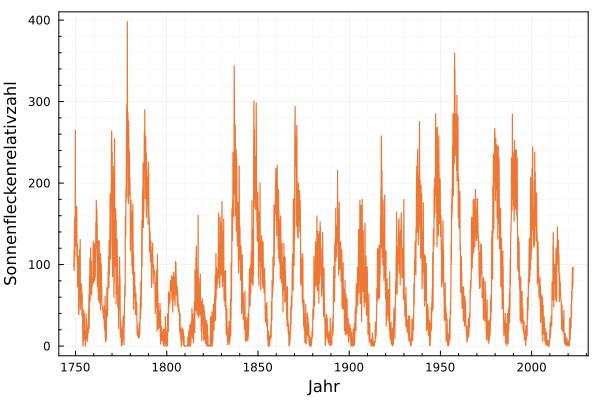
\includegraphics{./sonnenflecken_files/figure-pdf/cell-2-output-1.svg}

}

\end{figure}

Wir versuchen nun, die offensichtlich vorhandene Periodizität zu
berechnen und nutzen dafür die Schnelle Fourietransformation
\texttt{FFT}.

\begin{Shaded}
\begin{Highlighting}[]
\ImportTok{using} \BuiltInTok{FFTW}
\ImportTok{using} \BuiltInTok{Statistics}
\NormalTok{S }\OperatorTok{=} \FunctionTok{fft}\NormalTok{(SN }\OperatorTok{.{-}} \FunctionTok{mean}\NormalTok{(SN))}
\FunctionTok{popfirst!}\NormalTok{(S)}
\FunctionTok{plot}\NormalTok{(}\FunctionTok{abs}\NormalTok{.(S), label}\OperatorTok{=}\StringTok{""}\NormalTok{)}
\FunctionTok{ylabel!}\NormalTok{(}\StringTok{"Amplitudenspektrum"}\NormalTok{)}
\end{Highlighting}
\end{Shaded}

\begin{figure}[H]

{\centering 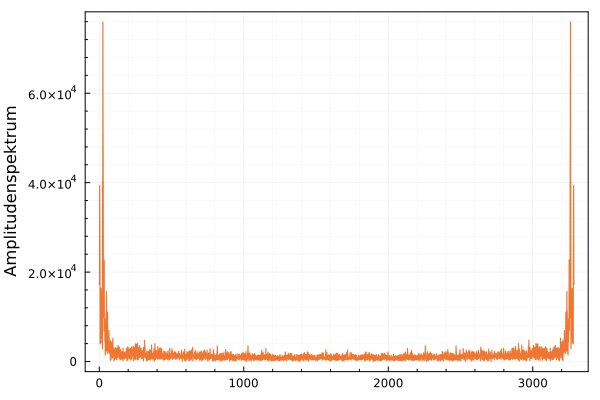
\includegraphics{./sonnenflecken_files/figure-pdf/cell-3-output-1.svg}

}

\end{figure}

\begin{Shaded}
\begin{Highlighting}[]
\NormalTok{n }\OperatorTok{=} \FunctionTok{length}\NormalTok{(S)}
\NormalTok{up }\OperatorTok{=} \FunctionTok{Int}\NormalTok{(}\FunctionTok{floor}\NormalTok{(n}\OperatorTok{/}\FloatTok{2}\NormalTok{))}
\NormalTok{power }\OperatorTok{=} \FunctionTok{abs}\NormalTok{.(S[}\FloatTok{1}\OperatorTok{:}\NormalTok{up, }\OperatorTok{:}\NormalTok{])}\OperatorTok{.\^{}}\FloatTok{2}
\NormalTok{samplinginterval }\OperatorTok{=} \FloatTok{1.0} \OperatorTok{/} \FloatTok{12.0}
\NormalTok{nyquist }\OperatorTok{=} \FloatTok{1} \OperatorTok{/}\NormalTok{ (}\FloatTok{2} \OperatorTok{*}\NormalTok{ samplinginterval)}
\NormalTok{freq }\OperatorTok{=}\NormalTok{ [}\FloatTok{1}\OperatorTok{:}\NormalTok{up}\OperatorTok{...}\NormalTok{] }\OperatorTok{./}\NormalTok{ (n }\OperatorTok{/} \FloatTok{2}\NormalTok{) }\OperatorTok{*}\NormalTok{ nyquist}
\FunctionTok{plot}\NormalTok{(freq, power)}
\FunctionTok{xlabel!}\NormalTok{(}\StringTok{"Frequenz in 1/a"}\NormalTok{)}
\FunctionTok{ylabel!}\NormalTok{(}\StringTok{"Powerspektrum"}\NormalTok{)}
\end{Highlighting}
\end{Shaded}

\begin{figure}[H]

{\centering 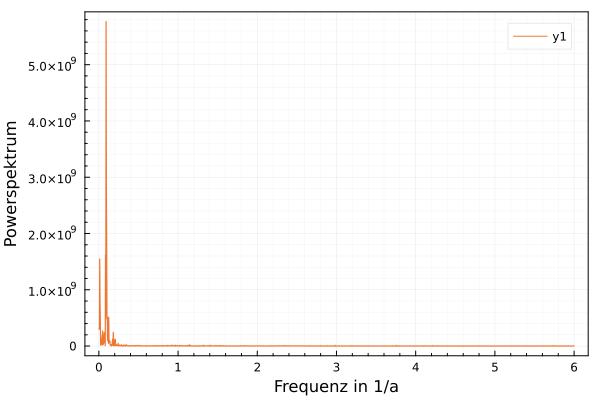
\includegraphics{./sonnenflecken_files/figure-pdf/cell-4-output-1.svg}

}

\end{figure}

\begin{Shaded}
\begin{Highlighting}[]
\NormalTok{period }\OperatorTok{=} \FloatTok{1} \OperatorTok{./}\NormalTok{ freq}
\NormalTok{i }\OperatorTok{=} \FunctionTok{argmax}\NormalTok{(power)}

\FunctionTok{plot}\NormalTok{(period, power, xscale}\OperatorTok{=:}\NormalTok{log10, label}\OperatorTok{=}\StringTok{""}\NormalTok{)}
\FunctionTok{scatter!}\NormalTok{([period[i]], [power[i]], m}\OperatorTok{=:}\NormalTok{o, label}\OperatorTok{=}\StringTok{""}\NormalTok{)}
\FunctionTok{xlabel!}\NormalTok{(}\StringTok{"Periodendauer in a"}\NormalTok{)}
\FunctionTok{ylabel!}\NormalTok{(}\StringTok{"Powerspektrum"}\NormalTok{)}
\FunctionTok{title!}\NormalTok{(}\StringTok{"Sonnenfleckenzyklus: }\SpecialCharTok{$}\NormalTok{(}\FunctionTok{round}\NormalTok{(period[i], digits}\OperatorTok{=}\FloatTok{2}\NormalTok{))}\StringTok{ a"}\NormalTok{)}
\end{Highlighting}
\end{Shaded}

\begin{figure}[H]

{\centering 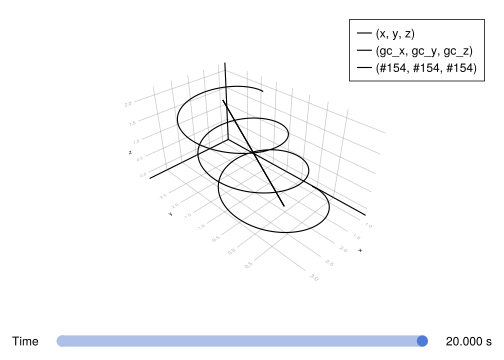
\includegraphics{./sonnenflecken_files/figure-pdf/cell-5-output-1.svg}

}

\end{figure}

\part{Plasmen und ihre Magnetfelder}

\hypertarget{plasmen}{%
\chapter{Plasmen}\label{plasmen}}

Der Begriff des Plasmas (von altgriechisch πλάσμα plásma) stammt aus dem
Griechischen und bedeutet \emph{das Gebildete, Geformte}.

Wir benutzen die folgende Definition:

\begin{tcolorbox}[enhanced jigsaw, opacitybacktitle=0.6, toprule=.15mm, colback=white, rightrule=.15mm, breakable, bottomrule=.15mm, toptitle=1mm, titlerule=0mm, arc=.35mm, colbacktitle=quarto-callout-important-color!10!white, leftrule=.75mm, opacityback=0, coltitle=black, colframe=quarto-callout-important-color-frame, bottomtitle=1mm, title=\textcolor{quarto-callout-important-color}{\faExclamation}\hspace{0.5em}{Wichtig}, left=2mm]

Ein Plasma ist ein quasineutrales Gas geladener und neutraler Teilchen
mit kollektivem Verhalten.

\end{tcolorbox}

Bewegen sich die geladenen Teilchen in einem Plasma, können sie lokale
Änderungen der Ladungsträgerdichte hervorrufen. Die Folge sind
elektrische Felder. Die Bewegung geladener Teilchen erzeugt elektrische
Ströme, die wiederum von Magnetfeldern begleitet werden. Diese
Feldeffekte beeinflussen die Bewegung geladener Teilchen in großen
Abständen.

Bewegungsmuster der Teilchen hängen nicht nur von lokalen Bedingungen,
sondern auch vom Zustand des Plasmas in entfernten Bereichen ab. Über
große Entfernungen wirksame elektromagnetische Kräfte führen dazu, dass
die Teilchen im Plasma simultan mit anderen interagieren.

Außerdem muss man unterscheiden zwischen Ladung-Ladung- und
Ladung-Neutralgas-Wechselwirkungen.

Die wichtigsten Phänomene im Zusammenhang mit dem kollektivem Verhalten
von Plasmen sind die Debye-Abschirmung sowie die Plasmafrequenz.

\hypertarget{typische-plasmen}{%
\section{Typische Plasmen}\label{typische-plasmen}}

Folgende Tabelle Tabelle~\ref{tbl-typen} gibt einen Überblick über
verschieden Plasmatypen und ihre Eigenschaften (Gibbon (2016)).

\hypertarget{tbl-typen}{}
\begin{longtable}[]{@{}lll@{}}
\caption{\label{tbl-typen}Plasmatypen}\tabularnewline
\toprule()
Typ & Elektronendichte (cm\(^{-3}\)) & Temperatur (eV) \\
\midrule()
\endfirsthead
\toprule()
Typ & Elektronendichte (cm\(^{-3}\)) & Temperatur (eV) \\
\midrule()
\endhead
Sterne & \(10^{26}\) & 2000 \\
Trägheitsfusion & \(10^{25}\) & 3000 \\
Magnetische Fusion & \(10^{15}\) & 1000 \\
Laser-generiert & \(10^{18}\) - \(10^{24}\) & 100-1000 \\
Entladung & \(10^{12}\) & 1-10 \\
Ionosphäre & \(10^{6}\) & 0.1 \\
Interstellarer Raum & 1 & 0.01 \\
\bottomrule()
\end{longtable}

(1 eV = 11600 K)

\begin{figure}

{\centering \includegraphics{./images/paste-B4955853.png}

}

\caption{\label{fig-typical-plasma}Dichte-Temperatur-Regime für typische
Plasmen (aus Thorne \& Blandford (2017))}

\end{figure}

\hypertarget{debye-luxe4nge}{%
\section{Debye-Länge}\label{debye-luxe4nge}}

Eine wichtige Eigenschaft von Plasmen ist ihre Fähigkeit, elektrische
Potentiale abzuschirmen.

Debye \& Hückel (1923a) und Debye \& Hückel (1923b) vermitteln
grundlegende Theorien zu den Wechselwirkungen von Ionen in Elektrolyten.
Diese Erkenntnisse lassen sich auf Plasmen übertragen.

\begin{figure}

{\centering \includegraphics[width=5.83333in,height=\textheight]{./images/paste-718770F4.png}

}

\caption{\label{fig-elektrolyt}Debye-Abschirmung von geladenen Kugeln in
einem Plasma (aus Gibbon (2016))}

\end{figure}

\hypertarget{herleitung}{%
\subsection{Herleitung}\label{herleitung}}

Jedes geladene Teilchen innerhalb eines Plasmas zieht andere Teilchen
mit entgegengesetzter Ladung an und stößt Teilchen mit der gleichen
Ladung ab, wodurch in der unmittelbaren Umgebung des Teilchens eine
Wolke aus überwiegend entgegengesetzten Ladungen entsteht.

Diese Wolke schirmt die eigene Ladung des Teilchens von der Außenwelt
ab, d.~h. sie bewirkt, dass das Coulomb-Feld des Teilchens bei großen
Entfernungen exponentiell abnimmt, anstatt mit \(1/r^2\).

Diese Debye-Abschirmung der Ladung eines Teilchens kann wie folgt
demonstriert und quantifiziert werden (Thorne \& Blandford (2017)):

Man betrachte eine einzelne Testladung \(Q\) im Ursprung, die von einem
Plasma aus Protonen und Elektronen umgeben ist. Wir definieren mit
\(n_p(r)\) und \(n_e(r)\) die mittleren Dichten für Elektronen und
Protonen als glatte Funktionen des Abstandes \(r\) von der Testladung,
und mit \(\bar n\) die mittleren Dichten von Elektronen und Protonen.
Dann ist das elektrostatische Potential \(\Phi(r)\) außerhalb des
Teilchens Lösung der Poisson-Gleichung

\begin{equation}\protect\hypertarget{eq-poisson}{}{
-\nabla^2 \Phi = \frac{n_p - n_e}{\epsilon_0} e + \frac{Q}{\epsilon_0} \delta(r)
}\label{eq-poisson}\end{equation}

Wir bezeichnen die Ladung eines Protons mit \(+e\) und die Ladung des
Elektrons mit \(-e\).

Ein Proton besitzt in der Entfernung \(r\) von der Testladung das
elektrostatische Potential \(e \Phi(r)\).

Die mittlere Ladungsträgerdichte ändert sich entsprechend zu

\[
n_p(r) = \bar n \, e^{-\dfrac{e \Phi(r)}{kT}} \approx \bar n \left(1 - \frac{e \Phi}{k T} \right)
\]

bzw.

\[
n_e(r) = \bar n \, e^{+\dfrac{e \Phi(r)}{kT}} \approx \bar n \left(1 + \frac{e \Phi}{k T} \right).
\]

Damit wird Gleichung~\ref{eq-poisson} eine \emph{nichtlineare
Differentialgleichung} in \(\Phi\), weil \(n_p\) und \(n_e\) Funktionen
von \(\Phi\) sind.

Wir können aber wegen \(e\Phi \ll kT\) die Exponentialfunktion in eine
Taylorreihe entwickelt und Terme höherer Ordnung vernachlässigen.

Einsetzen in Gleichung~\ref{eq-poisson} liefert nach Linearisierung

\[
-\nabla^2 \Phi + \frac{2 \bar n e^2}{\epsilon_0 k T} \Phi = \frac{Q}{\epsilon_0}\delta(r).
\]

Die kugelsymmetrische (nur von \(r\) abhängige) Lösung ist

\[
\Phi(r) = \frac{Q}{4 \pi \epsilon_0 r} \, e^{-\sqrt{\dfrac{2r^2}{\lambda_D^2}}}
\]

und besitzt die Form eines Coulomb-Potentials mit exponentiellem Abfall.
Die charakteristische Skalenlänge dieses Abfalls ist der
\emph{Debye-Radius}

\[
\lambda_D = \sqrt{ \frac{\epsilon_0 k T}{\bar n e^2}}
\]

und ist ein Maß für die Größe der Debye-Abschirmung. Der Debye-Radius
hängt gleichermaßen von der Temperatur als auch von der Teilchendichte
des Plasmas ab. In einem idealen Plasmsa befinden sich viele Teilchen
innerhalb einer Kugel vom Radius \(\lambda_D\). Die Anzahl ist

\[
N_D = n_e \frac{4 \pi}{3} \lambda_D^3 \gg 1.
\]

\begin{figure}

{\centering \includegraphics[width=2.1875in,height=\textheight]{./images/paste-D4D1A82B.png}

}

\caption{\label{fig-ionenverteilung}Ionenverteilung in einer Lösung (aus
Wikipedia: Debye-Länge)}

\end{figure}

Wird eine Störung (z.B. eine Überschussladung) in ein Plasma
eingebracht, so reicht die Wirkung dieser Störung nur bis zu einer
Entfernung der Größenordnung \(\lambda_D\). Nur innerhalb dieses
Abstandes weicht die lokale Ladungsträgerdichte signifikant von der
makroskopischen elektrischen Neutralität ab
(Abbildung~\ref{fig-ionenverteilung}).

\hypertarget{beispiel}{%
\subsubsection{Beispiel}\label{beispiel}}

Im Allgemeinen ist \(\lambda_D\) sehr klein. In der Ionosphäre ist
\(n_e = 10^{12}\) m\(^{-3}\) und \(T=10^3\) K. Damit ist
\(\lambda_D = 10^{-3}\) m.

\begin{figure}

{\centering \includegraphics{./images/paste-2A0EC69D.png}

}

\caption{\label{fig-tabelle201}Typische Plasmaparameter (aus Thorne \&
Blandford (2017))}

\end{figure}

Die Tabelle in Abbildung~\ref{fig-tabelle201} gibt für typische Plasmen
die folgenden charakteristischen Größen an:

\begin{itemize}
\tightlist
\item
  Teilchendichte der Elektronen \(n_e\)
\item
  Temperatur T
\item
  Magnetfeld \(B\)
\item
  Debye-Länge \(\lambda_D\)
\item
  Debye-Zahl \(N_D\)
\item
  Plasmafrequenz \(\omega_p\)
\item
  \(\nu_{ee}\)
\item
  Larmor-Kreisfrequenz \(\omega_c\)
\item
  Larmor-Radius \(r_L\).
\end{itemize}

\hypertarget{plasmaschwingungen-und-plasmafrequenz}{%
\section{Plasmaschwingungen und
Plasmafrequenz}\label{plasmaschwingungen-und-plasmafrequenz}}

Das wichtigste dynamische Phänomen in Plasmen ist die
Schwingungsbewegung von Protonen und Elektronen relativ zueinander.

Wird ein Plasma plötzlich aus seinem Gleichgewichtszustand gebracht,
verursachen die internen Raumladungsfelder kollektive
Partikelbewegungen, welche anstreben, die ursprüngliche
Ladungsneutralität wiederherzustellen.

Diese kollektiven Schwingungsmuster laufen mit einer bestimmten
\emph{Plasma-Frequenz} ab. Wegen der hohen Frequenz tragen die
Elektroden aufgrund ihrer im Vergleich zu Protonen geringeren
Massenträgheit maßgeblich zur Plasmaschwingung bei. Elektronen schwingen
kollektiv um die schweren Ionen, wobei die Rückstellkräfte durch die
Ion-Elektron-Coulomb-Kräfte verursacht werden. Die Periodendauer dieser
Bewegung ist eine typische Zeitskala.

\begin{figure}

{\centering \includegraphics{./images/paste-1FB78BDE.png}

}

\caption{\label{fig-osz}Schematische Darstellung der Verschiebung von
Elektronen relativ zu Protonen während einer Plasmaschwingung (aus
Thorne \& Blandford (2017))}

\end{figure}

\hypertarget{herleitung-1}{%
\subsection{Herleitung}\label{herleitung-1}}

Wir platzieren das Plasma gemäß Abb. Abbildung~\ref{fig-osz} entlang
einer unendlich ausgedehnten Ebene in \(x=0\) und nehmen an, dass alle
Protonen ortsfest bleiben. Die Elektronen werden relativ zu den Protonen
um den Betrag \(\xi_0\) nach rechts in \(x\)-Richtung verschoben. Wir
beobachten die Flächenüberschussladungsdichten \(-e \bar n \xi_0\) am
rechten Ende des Plasmas, sowie \(+e \bar n \xi_0\) am linken Ende des
Plasmas. Das resultierende elektrische Feld im Innern des Plasmas zum
Zeitpunkt \(t=0\) ist \(\mathbf E = (E, 0, 0)^\top\), also

\[
E = \frac{e \bar n \xi_0}{\epsilon_0}.
\]

Dieses Feld übt eine Coulomb-Kraft auf die Protonen und Elektronen aus.
Die Bewegungsgleichung für die Veschiebung lautet

\[
\ddot \xi = - \frac{e}{m_e} E = - \frac{e^2 \bar n}{\epsilon_0 m_e} \xi.
\]

Dies ist eine \emph{harmonische Schwingungsdifferentialgleichung}. Wir
haben wegen des Masseverhältnisses von Elektronen zu Protonen
\(m_e/m_p = 1 / 1836\) die Kraftwirkung auf die Protonen vernachlässigt.

Mit der oben angegebene Anfangsbedingung für \(t=0\) schwingen die
Elektronen harmonisch mit den Ortskoordinaten

\[
\xi(t) = \xi_0 \cos(\omega_p t),
\]

wobei die Plasmafrequenz

\[
\omega_p = \sqrt{ \frac{\bar n e^2}{\epsilon_0 m_e} }
\]

nur von der Plasmadichte \(\bar n\) aber \emph{nicht} von der Temperatur
\(T\) oder der magnetischen Feldstärke abhängt.

Die thermische Geschwindigkeit der Elektronen ist definiert durch

\[
v_e = \sqrt{ \frac{k T}{m_e} },
\]

somit ist

\[
\omega_p = \frac{v_e}{\lambda_D}.
\]

Mit anderen Worten: Thermische Elektronen legen innerhalb einer
Plasmaschwingungsperiode etwa eine Debye-Länge zurück.

\hypertarget{newtonsche-bewegungsgleichung}{%
\chapter{Newtonsche
Bewegungsgleichung}\label{newtonsche-bewegungsgleichung}}

Die Bewegung geladener Teilchen in einem stark verdünnten Plasma lässt
sich bei Vernachlässigung von Stößen durch eine Einzelteilchentheorie
gut annähern.

Die Änderung des Bewegungszustandes eines Teilchen wird durch die
\emph{Newtonsche Bewegungsgleichung} formuliert. Die Newtonsche Mechanik
beschreibt die klassische Teilchenbewegung als eine \emph{Bahn} durch
den Euklidischen Raum und die Zeit \(t\). Zum Zeitpunkt \(t\) befindet
sich das Teilchen am Ort \(\mathbf r(t)\). Die Funktion \(\mathbf r(t)\)
beschreibt die Bahn des Teilchens im Raum. Die Teilchengeschwindigkeit
\(\mathbf v(t)\) ist die Zeitableitung der Position. Der Impuls
\(\mathbf p(t)\) ist das Produkt aus Masse \(m\) und Geschwindigkeit
\(\mathbf v(t)\). Die Zeitableitung der Geschwindigkeit ist die
Beschleunigung \(\mathbf a(t)\).

Newtons zweites Grundgesetz der Mechanik \emph{lex secunda} besagt
folgendes:

\begin{quote}
Die Änderung der Bewegung ist der Einwirkung der bewegenden Kraft
proportional und geschieht nach der Richtung derjenigen geraden Linie,
nach welcher jene Kraft wirkt.
\end{quote}

Die Änderung des Bewegungszustandes kann nur unter Wirkung von Kräften
erfolgen. Werden diese Kräfte z.B. durch ein magnetisches Feld
\(\mathbf B\), ein elektrisches Feld \(\mathbf E\) sowie ein weiteres
Kraftfeld \(\mathbf F\) erzeugt, dann nimmt die Newtonsche
Bewegungsgleichung folgende Form an:

\begin{equation}\protect\hypertarget{eq-newton}{}{
m \ddot{\mathbf r} = q (\mathbf E + \mathbf v \times \mathbf B) + \mathbf F
}\label{eq-newton}\end{equation} Diese Gleichung kann für einfache
Feldkonfigurationen trivial integriert werden. Im Falle des
geomagnetischen Feldes gibt es keine geschlossenen Lösungen, sondern nur
Näherungen. Für Teilchen mit geringer Energie, wie sie bspw. in der
Ionosphäre oder im Van-Allen-Gürtel vorliegen, steht eine Theorie zur
Approximation bereit.

Zunächst werden wir Lösungen von Gleichung~\ref{eq-newton} für
vereinfachte Bedingungen betrachten. Später werden wir sehen, dass im
Allgemeinen von den Teilchen eine schnelle Kreisbewegung ausgeführt
wird, die überlagert wird durch die Bewegung durch Magnetfelder und
elektrische Felder.

Bei Anwesenheit eines Magnetfeldes bewegen sich geladene Teilchen in
Schraubenlinien entlang der Feldlinien. Die Bewegungsgleichung für ein
mit der Geschwindigkeit \(\mathbf v\) bewegtes Teilchen der Masse \(m\)
und Ladung \(q\) im Magnetfeld \(\mathbf B\) lautet \[
m \frac{d \mathbf v}{d t} = q \mathbf v \times \mathbf B
\]

Wir betrachten zunächst den Fall eines homogenen Magnetfeldes und setzen
\[
\mathbf B = const, \quad \mathbf E = 0, \quad \mathbf F = 0
\] Die Geschwindigkeit \(\mathbf v\) zerlegen wir vektoriell in eine
Komponente parallel und eine Komponente senkrecht zum magnetischen Feld.
\[
\mathbf v = \mathbf v_\| + \mathbf v_\perp
\] Gilt \(\mathbf v_\| = const\), dann ist \(m \dot{\mathbf v}_\| = 0\)
und \[
m \dot{\mathbf v}_\perp = q \mathbf v_\perp \times \mathbf B.
\]

\hypertarget{energieerhaltung}{%
\section{Energieerhaltung}\label{energieerhaltung}}

An dieser Stelle klären wir, ob die kinetische Energie des Teilchens
eine Erhaltungsgröße ist. Da \(\mathbf v_\| = const\), betrachten wir
die Änderung der kinetischen Energie \[
\frac{d E_{kin}}{d t} = \frac{d}{dt} \left( \frac{1}{2} m |\mathbf v_\perp|^2  \right) =
\mathbf v_\perp \cdot (m \dot{\mathbf v}_\perp) = q \mathbf v_\perp \cdot \left( \mathbf v_\perp \times \mathbf B \right) \overset{!}{=} 0.
\] Damit ist gezeigt, dass die kinetische Energie eines Teilchens im
Magnetfeld eine Erhaltungsgröße ist. Ein statisches Magnetfeld ändert
also weder \(\mathbf v\) noch die kinetische Energie. Dies ist eine sehr
wichtige Erkenntnis mit weitreichenden Konsequenzen für den Fall, dass
das Magnetfeld zeitlich variabel oder inhomogen ist.

\hypertarget{flugbahn}{%
\section{Flugbahn}\label{flugbahn}}

Bewegt sich das Teilchen in einer Ebene senkrecht zu \(\mathbf B\), dann
gilt \[
\mathbf v _\| \times \mathbf B = \mathbf 0
\] und \[
\mathbf v_\perp \times \mathbf B \perp \mathbf B.
\] Es gilt wegen \(\mathbf v = \mathbf \omega \times \mathbf r\)
(Bahngeschwindigkeit gleich Kreuzprodukt aus Winkelgeschwindigkeit und
Ortsvektor) \begin{equation}\protect\hypertarget{eq-gyration}{}{
\dot{\mathbf v}_\perp = \frac{q}{m} \left( \mathbf v_\perp \times \mathbf B \right) = \boldsymbol \omega_g \times \mathbf v_\perp
}\label{eq-gyration}\end{equation} Die Größe \(\mathbf \omega_g\) ist
die vektorielle Winkelgeschwindigkeit der Kreisbewegung. Es folgt \[
\boldsymbol \omega_g = - \frac{q}{m} \mathbf B = 
\frac{|q|}{m} B \, \widehat{\boldsymbol \omega}_g =
\omega_g \widehat{\boldsymbol \omega}_g
\] Der Betrag der Winkelgeschwindigkeit wird als Zyklotronfrequenz (oder
Larmorfrequenz) bezeichnet. \(\widehat{\mathbf \omega}_g\) ist der
Einheitsvektor der Winkelgeschwindigkeit. Mit der Rechte-Hand-Regel
ergibt sich die Bewegungsrichtung. Die Richtung der Kreisbewegung hängt
vom Vorzeichen der Ladung des Teilchen ab. Es gilt \[
q < 0: \qquad \widehat{\boldsymbol \omega}_g \| \mathbf B \qquad \text{parallel}
\] \[
q > 0: \qquad -\widehat{\boldsymbol \omega}_g \| \mathbf B \qquad \text{antiparallel}
\] Integrieren wir Gleichung~\ref{eq-gyration} zeitlich, erkennen wir
den Zusammenhang zwischen Bahngeschwindigkeit und Teilchenposition. Es
gilt \[
\mathbf v_\perp = \boldsymbol \omega_g \times \mathbf r_g
\] Mit \(\mathbf r_g\) bezeichnen wir die Teilchenposition. Sie
beschreibt eine Kreisbahn mit Radius \(r_g\) um den
Gyrationsmittelpunkt, der auch als \emph{Führungszentrum} bezeichnet
wird.

\hypertarget{beispiel-1}{%
\subsection{Beispiel}\label{beispiel-1}}

Wir berechnen die Zyklotronfrequenz und den Gyratonsradius für ein
Elektron. Die Elektronenmasse ist \[
m_e = 9.109 \times 10^{-31} ~\text{kg},
\] seine Ladung entspricht der Elementarladung \[
|q| = e = 1.602 \times 10^{-19} ~ \text{C}.
\] Wird \(\mathbf B\) in Tesla angegeben, gilt für die Zyklotronfrequenz
des Elektrons die Gleichung \[
\omega_c^e = \frac{e B}{m_e} = 1.76 \times 10^{11} \, B \text{ in rad}\cdot s^{-1}
\] Da Protonen eine um den Faktor 1890 größere Masse als Elektronen
besitzen, ist ihre Zyklotronfrequenz niedriger: \[
\omega_c^p = \frac{e B}{m_p} = 9.58 \times 10^{7} \, B \text{ in rad}\cdot s^{-1}
\] Der Gyrationsradius ist \[
r_g = \frac{v_\perp}{\omega_g} = \frac{m v_\perp}{|q| B}.
\]

\hypertarget{proton-und-elektron}{%
\chapter{Proton und Elektron}\label{proton-und-elektron}}

\begin{Shaded}
\begin{Highlighting}[]
\ImportTok{using} \BuiltInTok{TestParticle}
\ImportTok{using} \BuiltInTok{Meshes}
\ImportTok{using} \BuiltInTok{OrdinaryDiffEq}
\ImportTok{using} \BuiltInTok{Plots}
\ImportTok{using} \BuiltInTok{Markdown}
\FunctionTok{theme}\NormalTok{(}\OperatorTok{:}\NormalTok{vibrant)}
\FunctionTok{default}\NormalTok{(widen}\OperatorTok{=}\ConstantTok{false}\NormalTok{)}

\KeywordTok{function} \FunctionTok{circle}\NormalTok{(radius, center, N)}
\NormalTok{    θ }\OperatorTok{=} \FunctionTok{range}\NormalTok{(}\FloatTok{0}\NormalTok{, }\FloatTok{2}\NormalTok{π, N)}
\NormalTok{    center[}\FloatTok{1}\NormalTok{] }\OperatorTok{.+}\NormalTok{ radius }\OperatorTok{*} \FunctionTok{cos}\NormalTok{.(θ), center[}\FloatTok{2}\NormalTok{] }\OperatorTok{.+}\NormalTok{ radius }\OperatorTok{*} \FunctionTok{sin}\NormalTok{.(θ)}
\KeywordTok{end}
\end{Highlighting}
\end{Shaded}

\begin{verbatim}
circle (generic function with 1 method)
\end{verbatim}

Wir betrachten den Fall, dass das Teilchen mit der Geschwindigkeit
\(\mathbf v = \mathbf v_\perp\) in ein Magnetfeld \(\mathbf B\) und
elektrisches Feld \(\mathbf E\) eingebracht wird.

Die Bewegungsgleichung lautet \[
\dot{\mathbf v}_\perp = \frac{q}{m} \left( \mathbf E +  \mathbf v_\perp \times \mathbf B \right)
\]

Vereinfachend nehmen wir zunächst an, dass \(\mathbf E = \mathbf 0\).
Weiterhin sei \(\mathbf B = (0, 0, B)^\top\) homogen.

Aus der Lösung berechnen wir die Kreisfrequenz der Gyrationsbewegung \[
\omega_g = \frac{|q| B}{m}
\] und den Gyrationsradius \[
r_g = \frac{m v_\perp}{|q| B}.
\]

\hypertarget{numerisches-beispiel}{%
\section{Numerisches Beispiel}\label{numerisches-beispiel}}

Wir berechnen die Gyrationsfrequenz und den Gyrationsradius für
nichtrelativistische Elektronen und Protonen. Die Ladung eines Protons
beträgt \(q = +e = +1.60217662 \times 10^{-19}\) C, seine Masse ist
\(1.673557546 \times 10^{-27}\) kg. Die Ladung eines Elektrons beträgt
\(q = -e = -1.60217662 \times 10^{-19}\) C, seine Masse ist
\(9.10938356 \times 10^{-31}\) kg.

Im Magnetfeld der Stärke \(B = 1\) nT erhalten wir für die
Gyrationsfrequenz \[
f_g = \frac{\omega_g}{2 \pi} = \frac{|q| B}{2 \pi m}
\]

\begin{Shaded}
\begin{Highlighting}[]
\NormalTok{m\_p }\OperatorTok{=}\NormalTok{ TestParticle.mᵢ}
\NormalTok{m\_e }\OperatorTok{=}\NormalTok{ TestParticle.mₑ}
\NormalTok{q\_p }\OperatorTok{=}\NormalTok{ TestParticle.qᵢ}
\NormalTok{q\_e }\OperatorTok{=}\NormalTok{ TestParticle.qₑ}
\NormalTok{B }\OperatorTok{=} \FloatTok{1.0e{-}9}
\NormalTok{v }\OperatorTok{=} \FloatTok{1.0}

\NormalTok{f\_p }\OperatorTok{=}\NormalTok{ q\_p }\OperatorTok{*}\NormalTok{ B }\OperatorTok{/}\NormalTok{ (}\FloatTok{2} \OperatorTok{*} \ConstantTok{pi} \OperatorTok{*}\NormalTok{ m\_p) }
\NormalTok{f\_e }\OperatorTok{=} \FunctionTok{abs}\NormalTok{(q\_e) }\OperatorTok{*}\NormalTok{ B }\OperatorTok{/}\NormalTok{ (}\FloatTok{2} \OperatorTok{*} \ConstantTok{pi} \OperatorTok{*}\NormalTok{ m\_e) }

\NormalTok{r\_p }\OperatorTok{=}\NormalTok{ m\_p }\OperatorTok{*}\NormalTok{ v }\OperatorTok{/} \FunctionTok{abs}\NormalTok{(q\_p) }\OperatorTok{/}\NormalTok{ B}
\NormalTok{r\_e }\OperatorTok{=}\NormalTok{ m\_e }\OperatorTok{*}\NormalTok{ v }\OperatorTok{/} \FunctionTok{abs}\NormalTok{(q\_e) }\OperatorTok{/}\NormalTok{ B}

\NormalTok{Markdown.}\FunctionTok{parse}\NormalTok{(}\StringTok{"""}
\StringTok{Die Gyrationsfrequenz für Protonen beträgt }\SpecialCharTok{$}\NormalTok{(}\FunctionTok{round}\NormalTok{(f\_p, digits}\OperatorTok{=}\FloatTok{3}\NormalTok{))}\StringTok{ Hz.}
\StringTok{Die Gyrationsfrequenz für Elektronen beträgt }\SpecialCharTok{$}\NormalTok{(}\FunctionTok{round}\NormalTok{(f\_e, digits}\OperatorTok{=}\FloatTok{3}\NormalTok{))}\StringTok{ Hz.}
\StringTok{Der Gyrationsradius für Protonen beträgt }\SpecialCharTok{$}\NormalTok{(}\FunctionTok{round}\NormalTok{(r\_p, sigdigits}\OperatorTok{=}\FloatTok{3}\NormalTok{))}\StringTok{ m.}
\StringTok{Der Gyrationsradius für Elektronen beträgt }\SpecialCharTok{$}\NormalTok{(}\FunctionTok{round}\NormalTok{(r\_e, sigdigits}\OperatorTok{=}\FloatTok{3}\NormalTok{))}\StringTok{ m.}
\StringTok{"""}\NormalTok{)}
\end{Highlighting}
\end{Shaded}

Die Gyrationsfrequenz für Protonen beträgt 0.015 Hz. Die
Gyrationsfrequenz für Elektronen beträgt 27.992 Hz. Der Gyrationsradius
für Protonen beträgt 10.4 m. Der Gyrationsradius für Elektronen beträgt
0.00569 m.

\begin{Shaded}
\begin{Highlighting}[]
\NormalTok{x }\OperatorTok{=} \FunctionTok{range}\NormalTok{(}\OperatorTok{{-}}\FloatTok{20}\NormalTok{, }\FloatTok{20}\NormalTok{, length}\OperatorTok{=}\FloatTok{41}\NormalTok{)}
\NormalTok{y }\OperatorTok{=} \FunctionTok{range}\NormalTok{(}\OperatorTok{{-}}\FloatTok{20}\NormalTok{, }\FloatTok{20}\NormalTok{, length}\OperatorTok{=}\FloatTok{41}\NormalTok{)}
\NormalTok{z }\OperatorTok{=} \FunctionTok{range}\NormalTok{(}\OperatorTok{{-}}\FloatTok{20}\NormalTok{, }\FloatTok{20}\NormalTok{, length}\OperatorTok{=}\FloatTok{41}\NormalTok{)}
\NormalTok{B }\OperatorTok{=} \FunctionTok{fill}\NormalTok{(}\FloatTok{0.0}\NormalTok{, }\FloatTok{3}\NormalTok{, }\FunctionTok{length}\NormalTok{(x), }\FunctionTok{length}\NormalTok{(y), }\FunctionTok{length}\NormalTok{(z)) }\CommentTok{\# [T]}
\NormalTok{E }\OperatorTok{=} \FunctionTok{fill}\NormalTok{(}\FloatTok{0.0}\NormalTok{, }\FloatTok{3}\NormalTok{, }\FunctionTok{length}\NormalTok{(x), }\FunctionTok{length}\NormalTok{(y), }\FunctionTok{length}\NormalTok{(z)) }\CommentTok{\# [V/m]}
\NormalTok{B[}\FloatTok{3}\NormalTok{,}\OperatorTok{:}\NormalTok{,}\OperatorTok{:}\NormalTok{,}\OperatorTok{:}\NormalTok{] }\OperatorTok{.=} \FloatTok{1e{-}9}
\CommentTok{\# E[2,:,:,:] .= 1e{-}10}
\ConstantTok{nothing}
\end{Highlighting}
\end{Shaded}

\begin{Shaded}
\begin{Highlighting}[]
\NormalTok{Δx }\OperatorTok{=}\NormalTok{ x[}\FloatTok{2}\NormalTok{] }\OperatorTok{{-}}\NormalTok{ x[}\FloatTok{1}\NormalTok{]}
\NormalTok{Δy }\OperatorTok{=}\NormalTok{ y[}\FloatTok{2}\NormalTok{] }\OperatorTok{{-}}\NormalTok{ y[}\FloatTok{1}\NormalTok{]}
\NormalTok{Δz }\OperatorTok{=}\NormalTok{ z[}\FloatTok{2}\NormalTok{] }\OperatorTok{{-}}\NormalTok{ z[}\FloatTok{1}\NormalTok{]}

\NormalTok{grid }\OperatorTok{=} \FunctionTok{CartesianGrid}\NormalTok{((}\FunctionTok{length}\NormalTok{(x)}\OperatorTok{{-}}\FloatTok{1}\NormalTok{, }\FunctionTok{length}\NormalTok{(y)}\OperatorTok{{-}}\FloatTok{1}\NormalTok{, }\FunctionTok{length}\NormalTok{(z)}\OperatorTok{{-}}\FloatTok{1}\NormalTok{),}
\NormalTok{   (x[}\FloatTok{1}\NormalTok{], y[}\FloatTok{1}\NormalTok{], z[}\FloatTok{1}\NormalTok{]),}
\NormalTok{   (Δx, Δy, Δz))}
\ConstantTok{nothing}
\end{Highlighting}
\end{Shaded}

\begin{Shaded}
\begin{Highlighting}[]
\NormalTok{isAnalytic }\OperatorTok{=} \ConstantTok{false}
\NormalTok{trajectories }\OperatorTok{=} \FloatTok{1}

\NormalTok{x0 }\OperatorTok{=}\NormalTok{ [}\OperatorTok{{-}}\FloatTok{1.0}\NormalTok{, }\FloatTok{0.0}\NormalTok{, }\FloatTok{0.0}\NormalTok{] }\CommentTok{\# initial position, [m]}
\NormalTok{u0 }\OperatorTok{=}\NormalTok{ [}\FloatTok{0.0}\NormalTok{, }\FloatTok{1.0}\NormalTok{, }\FloatTok{0.0}\NormalTok{] }\CommentTok{\# initial velocity, [m/s]}
\NormalTok{stateinit }\OperatorTok{=}\NormalTok{ [x0}\OperatorTok{...}\NormalTok{, u0}\OperatorTok{...}\NormalTok{]}

\NormalTok{param\_electron }\OperatorTok{=} \FunctionTok{prepare}\NormalTok{(grid, E, B, species}\OperatorTok{=}\NormalTok{Electron)}
\NormalTok{tspan\_electron }\OperatorTok{=}\NormalTok{ (}\FloatTok{0.0}\NormalTok{, }\FloatTok{0.1}\NormalTok{)}

\NormalTok{param\_proton }\OperatorTok{=} \FunctionTok{prepare}\NormalTok{(grid, E, B, species}\OperatorTok{=}\NormalTok{Proton)}
\NormalTok{tspan\_proton }\OperatorTok{=}\NormalTok{ (}\FloatTok{0.0}\NormalTok{, }\FloatTok{200.0}\NormalTok{)}

\NormalTok{prob\_e }\OperatorTok{=} \FunctionTok{ODEProblem}\NormalTok{(trace!, stateinit, tspan\_electron, param\_electron)}
\NormalTok{prob\_p }\OperatorTok{=} \FunctionTok{ODEProblem}\NormalTok{(trace!, stateinit, tspan\_proton, param\_proton)}
\NormalTok{sol\_e }\OperatorTok{=} \FunctionTok{solve}\NormalTok{(prob\_e, }\FunctionTok{Tsit5}\NormalTok{(); save\_idxs}\OperatorTok{=}\NormalTok{[}\FloatTok{1}\NormalTok{,}\FloatTok{2}\NormalTok{,}\FloatTok{3}\NormalTok{])}
\NormalTok{sol\_p }\OperatorTok{=} \FunctionTok{solve}\NormalTok{(prob\_p, }\FunctionTok{Tsit5}\NormalTok{(); save\_idxs}\OperatorTok{=}\NormalTok{[}\FloatTok{1}\NormalTok{,}\FloatTok{2}\NormalTok{,}\FloatTok{3}\NormalTok{]);}
\end{Highlighting}
\end{Shaded}

\begin{Shaded}
\begin{Highlighting}[]
\FunctionTok{plot}\NormalTok{(sol\_e, idxs}\OperatorTok{=}\NormalTok{(}\FloatTok{1}\NormalTok{,}\FloatTok{2}\NormalTok{), lw}\OperatorTok{=}\FloatTok{3}\NormalTok{, label}\OperatorTok{=}\StringTok{"Elektron"}\NormalTok{)}

\NormalTok{c }\OperatorTok{=} \FunctionTok{circle}\NormalTok{(r\_e ,[}\OperatorTok{{-}}\FloatTok{1.0} \OperatorTok{{-}}\NormalTok{ r\_e; }\FloatTok{0.0}\NormalTok{], }\FloatTok{32}\NormalTok{);}
\FunctionTok{plot!}\NormalTok{(c[}\FloatTok{1}\NormalTok{], c[}\FloatTok{2}\NormalTok{], label}\OperatorTok{=}\StringTok{"analytisch"}\NormalTok{, lw}\OperatorTok{=}\FloatTok{0.5}\NormalTok{, aspect\_ratio}\OperatorTok{=:}\NormalTok{equal)}
\end{Highlighting}
\end{Shaded}

\begin{figure}[H]

{\centering 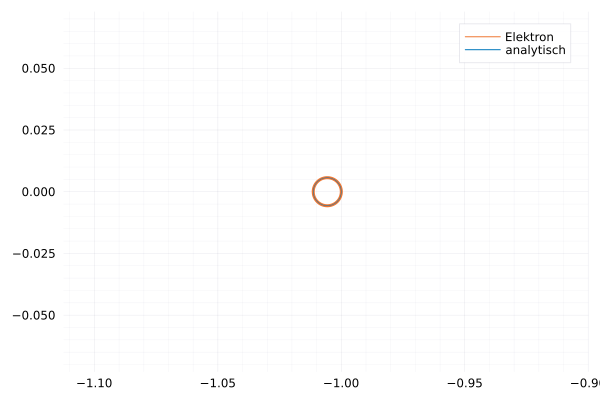
\includegraphics{./motion_homogen_files/figure-pdf/cell-7-output-1.svg}

}

\end{figure}

\begin{Shaded}
\begin{Highlighting}[]
\FunctionTok{plot}\NormalTok{(sol\_p, idxs}\OperatorTok{=}\NormalTok{(}\FloatTok{1}\NormalTok{,}\FloatTok{2}\NormalTok{), lw}\OperatorTok{=}\FloatTok{3}\NormalTok{, label}\OperatorTok{=}\StringTok{"Proton"}\NormalTok{)}

\NormalTok{c }\OperatorTok{=} \FunctionTok{circle}\NormalTok{(r\_p ,[}\OperatorTok{{-}}\FloatTok{1.0} \OperatorTok{+}\NormalTok{ r\_p; }\FloatTok{0.0}\NormalTok{], }\FloatTok{64}\NormalTok{);}
\FunctionTok{plot!}\NormalTok{(c[}\FloatTok{1}\NormalTok{], c[}\FloatTok{2}\NormalTok{], label}\OperatorTok{=}\StringTok{"analytisch"}\NormalTok{, lw}\OperatorTok{=}\FloatTok{0.5}\NormalTok{, aspect\_ratio}\OperatorTok{=:}\NormalTok{equal)}
\end{Highlighting}
\end{Shaded}

\begin{figure}[H]

{\centering 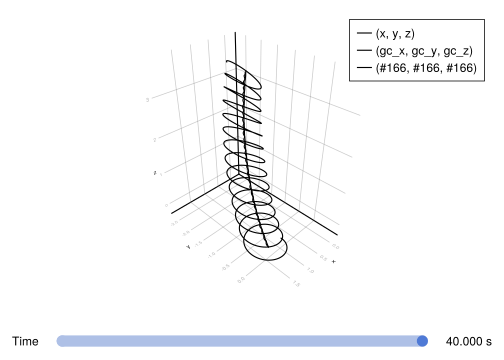
\includegraphics{./motion_homogen_files/figure-pdf/cell-8-output-1.svg}

}

\end{figure}

\hypertarget{simulation-der-teilchenbewegung-mit-julia}{%
\chapter{Simulation der Teilchenbewegung mit
Julia}\label{simulation-der-teilchenbewegung-mit-julia}}

Dieses Notebook demonstriert die numerische Simulation der
Teilchenbewegung.

Wir nutzen einen ODE-Löser des Julia-Pakets \emph{OrdinaryDiffEq}.
Außerdem nutzen wir \emph{TestParticle.jl}, ein Paket zum bequemen
Berechnen der Bewegungsbahnen geladener Teilchen in Dipolfeldern.

Die Visualisierung erfolgt mit \emph{Plots.jl}.

\begin{Shaded}
\begin{Highlighting}[]
\ImportTok{using} \BuiltInTok{TestParticle}
\ImportTok{using} \BuiltInTok{TestParticle}\NormalTok{: getB\_dipole, getE\_dipole, sph2cart, Rₑ}
\ImportTok{using} \BuiltInTok{OrdinaryDiffEq}
\ImportTok{using} \BuiltInTok{Plots}
\ImportTok{using} \BuiltInTok{Statistics}
\end{Highlighting}
\end{Shaded}

\begin{Shaded}
\begin{Highlighting}[]
\KeywordTok{function} \FunctionTok{fieldline}\NormalTok{(ϕ}\OperatorTok{::}\DataTypeTok{Float64}\NormalTok{, L}\OperatorTok{::}\DataTypeTok{Float64}\NormalTok{=}\FloatTok{2.5}\NormalTok{, nP}\OperatorTok{::}\DataTypeTok{Int}\NormalTok{=}\FloatTok{100}\NormalTok{)}

\NormalTok{   xyz }\OperatorTok{=}\NormalTok{ [ }\FunctionTok{sph2cart}\NormalTok{(}\FunctionTok{L*sin}\NormalTok{(θ)}\OperatorTok{\^{}}\FloatTok{2}\NormalTok{,ϕ,θ) for θ }\KeywordTok{in} \FunctionTok{range}\NormalTok{(}\OperatorTok{{-}}\ConstantTok{π}\NormalTok{,stop}\OperatorTok{=}\ConstantTok{π}\NormalTok{,length}\OperatorTok{=}\NormalTok{nP) ]}
\NormalTok{   x }\OperatorTok{=} \FunctionTok{Vector}\DataTypeTok{\{Float64\}}\NormalTok{(}\ConstantTok{undef}\NormalTok{,}\FunctionTok{length}\NormalTok{(xyz))}
\NormalTok{   y }\OperatorTok{=} \FunctionTok{Vector}\DataTypeTok{\{Float64\}}\NormalTok{(}\ConstantTok{undef}\NormalTok{,}\FunctionTok{length}\NormalTok{(xyz))}
\NormalTok{   z }\OperatorTok{=} \FunctionTok{Vector}\DataTypeTok{\{Float64\}}\NormalTok{(}\ConstantTok{undef}\NormalTok{,}\FunctionTok{length}\NormalTok{(xyz))}

   \ControlFlowTok{for}\NormalTok{ (i, pos) }\KeywordTok{in} \FunctionTok{enumerate}\NormalTok{(xyz)}
\NormalTok{      x[i],y[i],z[i] }\OperatorTok{=}\NormalTok{ [pos}\OperatorTok{...}\NormalTok{]}
   \ControlFlowTok{end}

\NormalTok{   (x,y,z)}
\KeywordTok{end}
\end{Highlighting}
\end{Shaded}

\begin{verbatim}
fieldline (generic function with 3 methods)
\end{verbatim}

\begin{Shaded}
\begin{Highlighting}[]
\KeywordTok{function} \FunctionTok{plot\_iso3d}\NormalTok{(xs, ys, zs; lw}\OperatorTok{=}\FloatTok{3}\NormalTok{, lc}\OperatorTok{=:}\NormalTok{red, title}\OperatorTok{=}\StringTok{"Isometric 3D plot"}\NormalTok{,label}\OperatorTok{=}\ConstantTok{false}\NormalTok{, camera}\OperatorTok{=}\NormalTok{(}\FloatTok{45}\NormalTok{,}\FloatTok{30}\NormalTok{))}
    \CommentTok{\# condition data for nearly isometric 3D plot }
\NormalTok{    x12, y12, z12 }\OperatorTok{=} \FunctionTok{extrema}\NormalTok{(xs), }\FunctionTok{extrema}\NormalTok{(ys), }\FunctionTok{extrema}\NormalTok{(zs)}
\NormalTok{    d }\OperatorTok{=} \FunctionTok{maximum}\NormalTok{([}\FunctionTok{diff}\NormalTok{([x12}\OperatorTok{...}\NormalTok{]),}\FunctionTok{diff}\NormalTok{([y12}\OperatorTok{...}\NormalTok{]),}\FunctionTok{diff}\NormalTok{([z12}\OperatorTok{...}\NormalTok{])])[}\FloatTok{1}\NormalTok{] }\OperatorTok{/} \FloatTok{2}
\NormalTok{    xm, ym, zm }\OperatorTok{=} \FunctionTok{mean}\NormalTok{(x12),  }\FunctionTok{mean}\NormalTok{(y12),  }\FunctionTok{mean}\NormalTok{(z12) }

    \CommentTok{\# plot data}
\NormalTok{    p }\OperatorTok{=}\NormalTok{ Plots.}\FunctionTok{plot}\NormalTok{(; xlabel}\OperatorTok{=}\StringTok{"x"}\NormalTok{,ylabel}\OperatorTok{=}\StringTok{"y"}\NormalTok{,zlabel}\OperatorTok{=}\StringTok{"z"}\NormalTok{, aspect\_ratio}\OperatorTok{=:}\NormalTok{equal, grid}\OperatorTok{=:}\ConstantTok{true}\NormalTok{)}
\NormalTok{    Plots.}\FunctionTok{plot!}\NormalTok{(xlims}\OperatorTok{=}\NormalTok{(xm}\OperatorTok{{-}}\NormalTok{d,xm}\OperatorTok{+}\NormalTok{d), ylims}\OperatorTok{=}\NormalTok{(ym}\OperatorTok{{-}}\NormalTok{d,ym}\OperatorTok{+}\NormalTok{d), zlims}\OperatorTok{=}\NormalTok{(zm}\OperatorTok{{-}}\NormalTok{d,zm}\OperatorTok{+}\NormalTok{d))}
\NormalTok{    Plots.}\FunctionTok{plot!}\NormalTok{(;camera}\OperatorTok{=}\NormalTok{camera)    }\CommentTok{\#(azimuth,elevation) ???}
\NormalTok{    Plots.}\FunctionTok{plot!}\NormalTok{(xs, ys, zs, title}\OperatorTok{=}\NormalTok{title,lw}\OperatorTok{=}\NormalTok{lw,lc}\OperatorTok{=}\NormalTok{lc,label}\OperatorTok{=}\NormalTok{label)}
\NormalTok{    Plots.}\FunctionTok{plot!}\NormalTok{(xs, ys, }\FunctionTok{zlims}\NormalTok{(p)[}\FloatTok{1}\NormalTok{] }\OperatorTok{.+} \FloatTok{0}\OperatorTok{*}\NormalTok{zs, lw}\OperatorTok{=}\FloatTok{1}\NormalTok{, lc}\OperatorTok{=:}\NormalTok{lightgray, label}\OperatorTok{=}\ConstantTok{false}\NormalTok{)}
\NormalTok{    Plots.}\FunctionTok{plot!}\NormalTok{(xs, }\FunctionTok{ylims}\NormalTok{(p)[}\FloatTok{2}\NormalTok{]  }\OperatorTok{.+} \FloatTok{0}\OperatorTok{*}\NormalTok{ys, zs, lw}\OperatorTok{=}\FloatTok{1}\NormalTok{, lc}\OperatorTok{=:}\NormalTok{lightgray, label}\OperatorTok{=}\ConstantTok{false}\NormalTok{)}
\NormalTok{    Plots.}\FunctionTok{plot!}\NormalTok{(}\FunctionTok{xlims}\NormalTok{(p)[}\FloatTok{1}\NormalTok{]  }\OperatorTok{.+} \FloatTok{0}\OperatorTok{*}\NormalTok{xs, ys, zs, lw}\OperatorTok{=}\FloatTok{1}\NormalTok{, lc}\OperatorTok{=:}\NormalTok{lightgray, label}\OperatorTok{=}\ConstantTok{false}\NormalTok{)}
\KeywordTok{end}
\end{Highlighting}
\end{Shaded}

\begin{verbatim}
plot_iso3d (generic function with 1 method)
\end{verbatim}

\begin{Shaded}
\begin{Highlighting}[]
\NormalTok{Ek }\OperatorTok{=} \FloatTok{5e7}

\NormalTok{m }\OperatorTok{=}\NormalTok{ TestParticle.mᵢ}
\NormalTok{q }\OperatorTok{=}\NormalTok{ TestParticle.qᵢ}
\NormalTok{c }\OperatorTok{=}\NormalTok{ TestParticle.c;}
\end{Highlighting}
\end{Shaded}

\begin{Shaded}
\begin{Highlighting}[]
\NormalTok{v₀ }\OperatorTok{=} \FunctionTok{sph2cart}\NormalTok{(}\FunctionTok{c*sqrt}\NormalTok{(}\FloatTok{1}\OperatorTok{{-}}\FloatTok{1}\OperatorTok{/}\NormalTok{(}\FloatTok{1}\OperatorTok{+}\NormalTok{Ek}\OperatorTok{*}\NormalTok{q}\OperatorTok{/}\NormalTok{(m}\OperatorTok{*}\NormalTok{c}\OperatorTok{\^{}}\FloatTok{2}\NormalTok{))}\OperatorTok{\^{}}\FloatTok{2}\NormalTok{), }\FloatTok{0.0}\NormalTok{, }\ConstantTok{π}\OperatorTok{/}\FloatTok{4}\NormalTok{)}
\CommentTok{\# initial position, [m]}
\NormalTok{r₀ }\OperatorTok{=} \FunctionTok{sph2cart}\NormalTok{(}\FloatTok{2.5}\OperatorTok{*}\NormalTok{Rₑ, }\FloatTok{0.0}\NormalTok{, }\ConstantTok{π}\OperatorTok{/}\FloatTok{2}\NormalTok{)}
\NormalTok{stateinit }\OperatorTok{=}\NormalTok{ [r₀}\OperatorTok{...}\NormalTok{, v₀}\OperatorTok{...}\NormalTok{]}
\CommentTok{\# obtain field}
\NormalTok{param }\OperatorTok{=} \FunctionTok{prepare}\NormalTok{(getE\_dipole, getB\_dipole)}
\NormalTok{tspan }\OperatorTok{=}\NormalTok{ (}\FloatTok{0.0}\NormalTok{, }\FloatTok{20.0}\NormalTok{);}
\end{Highlighting}
\end{Shaded}

\begin{Shaded}
\begin{Highlighting}[]
\NormalTok{prob }\OperatorTok{=} \FunctionTok{ODEProblem}\NormalTok{(trace\_analytic!, stateinit, tspan, param);}
\end{Highlighting}
\end{Shaded}

\begin{Shaded}
\begin{Highlighting}[]
\NormalTok{sol }\OperatorTok{=} \FunctionTok{solve}\NormalTok{(prob, }\FunctionTok{Tsit5}\NormalTok{(); save\_idxs}\OperatorTok{=}\NormalTok{[}\FloatTok{1}\NormalTok{,}\FloatTok{2}\NormalTok{,}\FloatTok{3}\NormalTok{])}

\NormalTok{x }\OperatorTok{=} \FunctionTok{getindex}\NormalTok{.(sol.u,}\FloatTok{1}\NormalTok{) }\OperatorTok{/}\NormalTok{ Rₑ}
\NormalTok{y }\OperatorTok{=} \FunctionTok{getindex}\NormalTok{.(sol.u,}\FloatTok{2}\NormalTok{) }\OperatorTok{/}\NormalTok{ Rₑ}
\NormalTok{z }\OperatorTok{=} \FunctionTok{getindex}\NormalTok{.(sol.u,}\FloatTok{3}\NormalTok{) }\OperatorTok{/}\NormalTok{ Rₑ;}
\end{Highlighting}
\end{Shaded}

\begin{Shaded}
\begin{Highlighting}[]
\FunctionTok{plot}\NormalTok{(x, y, z, aspect\_ratio}\OperatorTok{=:}\NormalTok{equal, legend}\OperatorTok{=}\ConstantTok{false}\NormalTok{)}
\ControlFlowTok{for}\NormalTok{ ϕ }\KeywordTok{in} \FunctionTok{range}\NormalTok{(}\FloatTok{0}\NormalTok{, stop}\OperatorTok{=}\FloatTok{2}\OperatorTok{*}\ConstantTok{π}\NormalTok{, length}\OperatorTok{=}\FloatTok{10}\NormalTok{)}
   \FunctionTok{plot!}\NormalTok{(}\FunctionTok{fieldline}\NormalTok{(ϕ)}\OperatorTok{...}\NormalTok{, color}\OperatorTok{=}\StringTok{"red"}\NormalTok{, aspect\_ratio}\OperatorTok{=:}\NormalTok{equal, alpha}\OperatorTok{=}\FloatTok{0.3}\NormalTok{, legend}\OperatorTok{=}\ConstantTok{false}\NormalTok{)}
\ControlFlowTok{end}

\FunctionTok{current}\NormalTok{()}
\end{Highlighting}
\end{Shaded}

\begin{figure}[H]

{\centering 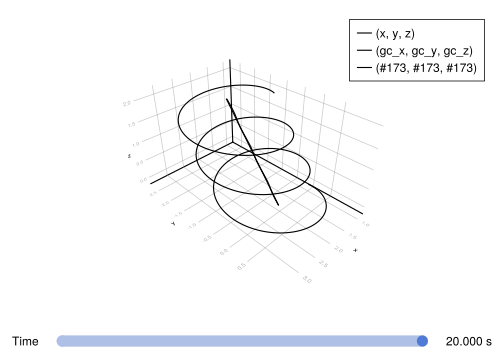
\includegraphics{./Dipolefield_Motion_files/figure-pdf/cell-9-output-1.pdf}

}

\end{figure}

\begin{Shaded}
\begin{Highlighting}[]
\NormalTok{p }\OperatorTok{=} \FunctionTok{plot\_iso3d}\NormalTok{(x, y, z, title}\OperatorTok{=}\StringTok{"Charged particle traces"}\NormalTok{)}
\NormalTok{p}
\end{Highlighting}
\end{Shaded}

\begin{figure}[H]

{\centering 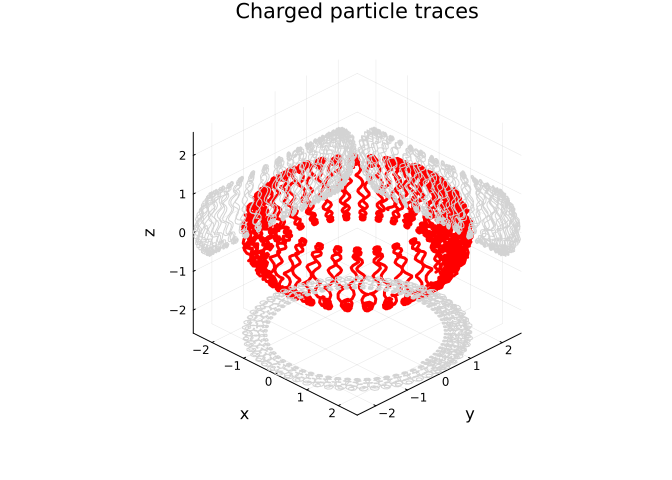
\includegraphics{./Dipolefield_Motion_files/figure-pdf/cell-10-output-1.pdf}

}

\end{figure}

\part{Die elektrische Leitfähigkeit der Ionosphäre}

\hypertarget{eej}{%
\chapter{EEJ}\label{eej}}

\part{Das erdmagnetische Außenfeld}

\hypertarget{ionosphuxe4re}{%
\chapter{Ionosphäre}\label{ionosphuxe4re}}

\hypertarget{variationen}{%
\chapter{Variationen}\label{variationen}}

\bookmarksetup{startatroot}

\hypertarget{phuxe4nomene-im-system-der-magnetosphuxe4re-und-ionosphuxe4re}{%
\chapter{Phänomene im System der Magnetosphäre und
Ionosphäre}\label{phuxe4nomene-im-system-der-magnetosphuxe4re-und-ionosphuxe4re}}

\bookmarksetup{startatroot}

\hypertarget{zusammenfassung}{%
\chapter{Zusammenfassung}\label{zusammenfassung}}

\bookmarksetup{startatroot}

\hypertarget{literaturverzeichnis}{%
\chapter*{Literaturverzeichnis}\label{literaturverzeichnis}}
\addcontentsline{toc}{chapter}{Literaturverzeichnis}

\markboth{Literaturverzeichnis}{Literaturverzeichnis}

\hypertarget{refs}{}
\begin{CSLReferences}{1}{0}
\leavevmode\vadjust pre{\hypertarget{ref-debye1923debye}{}}%
Debye, P. \& Hückel, E. (1923) On the Debye length in strong
electrolytes. \emph{Physikalische Zeitschrift}, \textbf{24}, 185.

\leavevmode\vadjust pre{\hypertarget{ref-debye1923theorie}{}}%
Debye, P. \& Hückel, E. (1923) {Zur Theorie der Elektrolyte. II. Das
Grenzgesetz f{ü}r die elektrische Leitf{ä}higkeit}. \emph{Physikalische
Zeitschrift}, \textbf{24}, 305--325.

\leavevmode\vadjust pre{\hypertarget{ref-gibbon}{}}%
Gibbon, P. (2016) Introduction to Plasma Physics. \emph{CERN Yellow
Reports}, Vol 1 (2016): Proceedings of the 2014 CAS--CERN Accelerator
School: Plasma Wake Acceleration, CERN, Geneva.
doi:\href{https://doi.org/10.5170/CERN-2016-001.51}{10.5170/CERN-2016-001.51}

\leavevmode\vadjust pre{\hypertarget{ref-kertz}{}}%
Kertz, W. (1971) {Einf{ü}hrung in die Geophysik II}.
\emph{Bibliographisches Institut, Mannheim}.

\leavevmode\vadjust pre{\hypertarget{ref-thorne2017modern}{}}%
Thorne, K.S. \& Blandford, R.D. (2017) \emph{Modern classical physics:
optics, fluids, plasmas, elasticity, relativity, and statistical
physics}, Princeton University Press.

\end{CSLReferences}



\end{document}
